% Unified theory of the relative GLV: one notation, one argument.
% Supersedes the \input of dmft_theory, appendix_dmft, zero_growth_theory, beta_theory and
% lifecycle_theory; those notes are kept as the record of how each result was obtained.
% Build: latexmk -pdf theory.tex   (from this directory)
\documentclass[11pt]{article}
\usepackage[a4paper,margin=25mm]{geometry}
\usepackage{amsmath,amssymb,amsthm,bm}
\usepackage{booktabs}
\usepackage{graphicx}
\graphicspath{{../../assets/figures/}{../zero_growth_theory/}}
\usepackage{float}
\usepackage{xcolor}
\usepackage{microtype}
\usepackage[hidelinks]{hyperref}
\usepackage[natbib=true,backend=bibtex]{biblatex}  % ponytail: local biber binary is broken (lipo); bibtex is enough here
\addbibresource{../../bib.bib}

\newcommand{\E}{\mathbb E}
\newcommand{\Var}{\operatorname{Var}}
\newcommand{\Cov}{\operatorname{Cov}}
\newcommand{\Sthr}{S_{\rm thr}}
\newcommand{\Dz}{\mathcal{D}z}
\newcommand{\PhiN}{\Phi_{\mathcal N}}
\newcommand{\phiN}{\phi_{\mathcal N}}
\newcommand{\bPhi}{\bar\Phi}
\newcommand{\bad}{\beta_{\rm ad}}
\newtheorem{proposition}{Proposition}
\newtheorem{corollary}{Corollary}

\title{Mean-field theory of the relative Lotka--Volterra economy\\[2pt]
\large Phases, growth, and the size--volatility relation}
\author{Ludovico Furlanetto}
\date{\today}

\begin{document}
\maketitle

\begin{abstract}
\noindent
We develop the theory of a generalised Lotka--Volterra (GLV) model of firms in which every
interaction is normalised by the mean firm size.  The normalisation makes the dynamics scale
invariant: the aggregate grows exponentially at a self-consistent rate, and the composition obeys
a disordered replicator equation.  A heterogeneous dynamical mean-field theory (HDMFT) on the
power-law interaction graph gives the phase diagram.  For an uncorrelated graph the loss of the
unique fixed point has a closed form, $\sigma_c\simeq\sqrt2\,[1-\tfrac12\Var\kappa\,(1-\mu^2/2\pi)]$ to
first order in the degree variance, while the zero-growth line hardly depends on the topology.
Above $\sigma_c$ trapping equilibria coexist with chaos.  In the fluctuating phase the fitness
felt by each firm is Gaussian, with mean and amplitude fixed by its degree, and independent
single firms driven by that fitness reproduce the size--volatility statistics of the network.
Under the unbalanced panel used empirically these statistics are set by firm life cycles.  The
one-firm equation is solvable for any fitness path; a firm exits on the first fitness dip
whose area exceeds an explicit threshold, which gives its lifetime law.  A firm's volatility is
its log range over its lifetime, and multiscaling follows from a general criterion: the growing
spread of lifetimes with size.  Each result is labelled as exact, leading order in $1/C$, or
numerical.
\end{abstract}

\tableofcontents

%======================================================================
\section{Introduction}
\label{sec:intro}

\paragraph{The facts.}
Let $v_i$ be the volatility of firm $i$'s growth rate and $\bar S_i$ its mean size.  In
Compustat the conditional moments scale as
\begin{equation}
  \E[v^q\mid\bar S]\sim\bar S^{-\zeta_q},\qquad \beta:=\zeta_1\approx0.2,\qquad
  \frac{\zeta_q}{\zeta_1}\approx2.0,\;2.6,\;2.9\quad(q=2,3,4),
  \label{eq:facts}
\end{equation}
so large firms are less volatile, but not as much as the $\bar S^{-1/2}$ of independent
subunits, and the ratio curve bends below the line $\zeta_q/\zeta_1=q$ of a volatility law of
fixed shape \citep{moran2024}.  We call the bend \emph{multiscaling}.  Simulations of the model
below reproduce both features.  This paper explains why, and maps where in parameter space
the model fluctuates and grows.

\paragraph{The argument in four steps.}
\begin{enumerate}
  \item \emph{Exact reductions} (Section~\ref{sec:model}).  Dividing the interactions by the mean
        size separates the scale from the composition.  The scale grows at $g(t)$; the
        composition is a replicator equation.  Each firm obeys a one-dimensional equation driven
        by its \emph{fitness} $\Phi_i(t)$, and its mean size equals its mean fitness.
  \item \emph{Mean-field theory and phase diagram} (Sections~\ref{sec:hdmft}--\ref{sec:fixed}).  At
        leading order in $1/C$ the fitness is a Gaussian process whose mean and amplitude depend
        on the degree through five order parameters.  The stability line of the unique fixed
        point and the zero-growth line follow in closed or nearly closed form; above the line
        trapping equilibria coexist with chaos.
  \item \emph{Single-firm reduction} (Section~\ref{sec:onefirm}).  In the fluctuating phase the
        size--volatility statistics of the full network are reproduced by independent single
        firms driven by Gaussian fitness with the mean-field law.  The network enters only
        through that law.
  \item \emph{Which firms are counted} (Sections~\ref{sec:panels}--\ref{sec:spells}).  A
        firm's volatility has two sources: fluctuations on its plateau, and the rise and fall
        that bracket its life.  The unbalanced panel used in the data is dominated by the second:
        exits are set by fitness dips whose area exceeds an explicit threshold, and the bend of
        the ratio curve is the growing spread of lifetimes with size.  The survivor panel, which
        sees only the plateau, is treated in the appendices.
\end{enumerate}
Table~\ref{tab:map} lists the results and their status.  ``Exact'' means it holds for the
finite-$N$ model.  ``Leading order'' means exact in the HDMFT, that is, at $N\to\infty$ and to
leading order in $1/C$.  ``Numerical'' means established by simulation and not derived.

\begin{table}[h]
\centering\small\setlength{\tabcolsep}{4pt}
\begin{tabular}{p{0.37\textwidth}p{0.36\textwidth}ll}
\toprule
result & statement & status & section\\
\midrule
scale--composition split & replicator with common drift $g(t)$ & exact & \ref{sec:split}\\
size is mean fitness & $\bar S_i=\bPhi_i$ for every stationary firm & exact & \ref{sec:firm}\\
fitness law & $\bPhi\mid\kappa$ Gaussian, amplitude $\propto\sqrt\kappa$ & leading order & \ref{sec:fitnesslaw}\\
chaos onset, regular graph & $\sigma_c=\sqrt2/(1+\gamma)$, independent of $\mu$ & leading order & \ref{sec:regular}\\
stability line, heterogeneous & $\sigma_c(\mu)$, closed form for bilinear kernel & leading order & \ref{sec:zerogrowth}\\
above $\sigma_c$ & trapping equilibria coexist with chaos & numerical & \ref{sec:above}\\
zero-growth line, power-law graph & $a=1$ in the HDMFT closure & leading order$^\dagger$ & \ref{sec:zerogrowth}\\
single-firm reduction & network $\to$ one firm in Gaussian fitness & numerical & \ref{sec:reduction}\\
adiabatic volatility law & $v=\sqrt D/S$, $\beta\to1$ at fixed degree & leading order & \ref{sec:adlaw}\\
sum rule & $\beta=\beta_A-\varepsilon_k$ & exact$^\ddagger$ & \ref{sec:sumrule}\\
survivor ensemble & degree channel $\varepsilon_k$ with no fitting & leading order & \ref{sec:ensemble}\\
multiscaling criterion & bend $\Leftrightarrow$ $\Var(\ln X\mid\bar S)$ grows & 2nd cumulant & \ref{sec:criterion}\\
lifetime identity & $v=\sqrt{\pi/2}\,(2\ell+V_p)/n$ & exact & \ref{sec:identity}\\
spells are humps & $V_p\simeq0$ below $8\tau$; merges add $\simeq0.7\ell$ & numerical & \ref{sec:humps}\\
exact one-firm solution & $1/S=\int e^{-[\mathcal A(t)-\mathcal A(t')]}dt'$ & exact & \ref{sec:rice}\\
lifetime law & $\bar L=\PhiN(u)/\nu(u)P_{\rm kill}(u)$ & leading order$^\S$ & \ref{sec:rice}\\
\bottomrule
\end{tabular}
\caption{Map of results.  $^\dagger$Controlled only below $\sigma\simeq1.02$; above, it is the
continuation of an unstable fixed point that agrees with simulation.  $^\ddagger$Given a
factorisation assumption stated with the result.  $^\S$Given the fitness law; checked in the one-firm process.}
\label{tab:map}
\end{table}

%======================================================================
\section{Model and exact reductions}
\label{sec:model}

\subsection{The model}

Firm $i=1,\dots,N$ has size $x_i(t)$, and $m(t)=N^{-1}\sum_jx_j$ is the mean size.  The relative
GLV is
\begin{equation}
  \dot x_i=x_i\left[1-\frac{x_i}{m}+\frac{1}{m}\sum_jW_{ij}x_j\right]+\lambda\,(m-x_i),
  \label{eq:model}
\end{equation}
with couplings on a graph of adjacency $A_{ij}$ and mean degree $C$,
\begin{equation}
  W_{ij}=A_{ij}\left(\frac{\mu}{C}+\frac{\sigma}{\sqrt C}z_{ij}\right),\qquad
  z_{ij}\sim\mathcal N(0,1),\qquad \overline{z_{ij}z_{ji}}=\gamma,\qquad W_{ii}=0 .
  \label{eq:couplings}
\end{equation}
This is the standard disordered-GLV scaling with one change: self-limitation and interactions
are measured in units of the mean size $m$ rather than of a fixed carrying capacity.  We use
$\mu<0$ for competition throughout, as in all figures.  The immigration term $\lambda(m-x_i)$
keeps every firm above a floor of order $\lambda m$ and acts as entry.

The graph is a configuration model with degree law $p(k)\propto k^{-\alpha}$, collapsed to a
simple graph.  Unless stated otherwise the production values are $N=8000$, $C=N/40=200$,
$\gamma=0$, $\lambda=10^{-3}$ and the operating point $(\mu,\sigma)=(-1.76,1.75)$, with
$\alpha\in\{2.2,2.5,3.5,6\}$; $\alpha=6$ is nearly homogeneous.  We write $\kappa=k/C$ for the
degree relative to the mean.

The right-hand side of \eqref{eq:model} is homogeneous of degree one in $x$: rescaling all sizes
rescales time derivatives by the same factor.  The overall scale is therefore a free direction.
It grows or shrinks exponentially, without the finite-time blow-up of the absolute GLV, and the
ratios $x_i/m$ carry all the structure.

\subsection{Scale and composition}
\label{sec:split}

Let $S_i=x_i/m$, so that $\langle S\rangle:=N^{-1}\sum_iS_i=1$.  Substituting $x_i=mS_i$ into
\eqref{eq:model} removes $m$ from every ratio,
\begin{equation}
  \dot m\,S_i+m\,\dot S_i=m\,S_iF_i+\lambda m(1-S_i),\qquad F_i:=1-S_i+(WS)_i .
  \label{eq:productrule}
\end{equation}
Averaging over $i$, with $\langle\dot S\rangle=0$ and the immigration term of zero mean,
\begin{equation}
  \frac{\dot m}{m}=g(t):=\langle SF\rangle=\sum_i\frac{x_i}{Nm}F_i .
  \label{eq:g}
\end{equation}
Inserting this back into \eqref{eq:productrule},
\begin{equation}
  \boxed{\;\dot S_i=S_i\bigl[F_i-g(t)\bigr]+\lambda(1-S_i),\qquad
  m(t)=m(0)\exp\!\int_0^tg(s)\,ds .\;}
  \label{eq:replicator}
\end{equation}
This is exact and equivalent to \eqref{eq:model}.  At $\lambda=0$ it is a replicator equation
with linear payoff, $F=\Pi S$ with $\Pi=-I+W+\mathbf 1\mathbf 1^T/N$ (using $\langle S\rangle=1$ to write
the constant as $\mathbf 1^TS/N$), and by Hofbauer's equivalence it is in turn a Lotka--Volterra
system of one dimension less \citep{hofbauer81}.

The drift $-g(t)$ is the mean-fitness subtraction of the replicator.  $g$ is the share-weighted
mean fitness of the economy and also its growth rate.  A firm gains share only if its fitness
beats this common field, and $g=\langle SF\rangle$ is exactly the value that preserves
$\langle S\rangle=1$.  Being an average over all firms, $g$ self-averages: its fluctuations are
$O(N^{-1/2})$, so in the mean-field limit it is a deterministic function of time.  The long-run
growth rate of the economy is $\bar g=\lim_{T\to\infty}T^{-1}\int_0^Tg$.

\subsection{One firm and its fitness}
\label{sec:firm}

Define the \emph{fitness} of firm $i$ as everything in its growth rate except its own
self-limitation,
\begin{equation}
  \Phi_i(t):=1-g(t)+(WS)_i(t).
\end{equation}
Then \eqref{eq:replicator} reads, exactly,
\begin{equation}
  \boxed{\;\frac{d\ln S_i}{dt}=\Phi_i(t)-S_i+\lambda\left(S_i^{-1}-1\right).\;}
  \label{eq:firm}
\end{equation}
This is a logistic equation with a moving carrying capacity.  When $\Phi_i>0$ the firm relaxes
towards $S_i=\Phi_i$ at rate $\approx S_i$; when $\Phi_i<0$ it decays at rate $|\Phi_i|$ down to the
immigration floor $S\approx\lambda/|\Phi_i|$, and climbs back when $\Phi_i$ turns positive.  In
simulation $\Phi_i(t)$ can be read off exactly by inverting \eqref{eq:firm}.

\begin{proposition}[Size is mean fitness; exact]\label{prop:size}
Over any window in which $\ln S_i$ starts and ends at the same value (or for $T\to\infty$ in a
stationary state),
\begin{equation}
  \bar S_i=\bPhi_i+\lambda\left(\overline{S_i^{-1}}-1\right)\simeq\bPhi_i ,
  \label{eq:sizefitness}
\end{equation}
where the bar is the window average and the correction is negligible above the floor.
\end{proposition}
\begin{proof}
Average \eqref{eq:firm}; the left side integrates to zero.
\end{proof}
In simulation $\bar S/\bPhi=1.000$ and $\mathrm{corr}(\bar S,\bPhi)=1.000$ for surviving firms on
every graph.  A firm is large because its environment is favourable on average, and its size is a
running estimate of that environment.

%======================================================================
\section{Heterogeneous dynamical mean-field theory}
\label{sec:hdmft}

\subsection{Degree classes and the structural cutoff}

Group the nodes into degree classes $p$ with population fractions $\rho_p$ and relative degrees
$v_p=k_p/N$, and let $P_{pr}$ be the probability that a node of class $p$ links to one of class
$r$.  With connectance $c=C/N$ the kernel must satisfy
\begin{equation}
  v_p=\sum_r\rho_rP_{pr},\qquad c=\sum_p\rho_pv_p .
  \label{eq:kernel}
\end{equation}
The uncorrelated choice $P_{pr}=v_pv_r/c$ exceeds one for pairs of hubs, $v_pv_r>c$: this is
the structural cutoff of a broad simple graph.  Following \citet{patil2026} we use the
soft-configuration kernel
\begin{equation}
  P_{pr}=\frac{h_ph_r}{h_ph_r+c},
  \label{eq:scm}
\end{equation}
with hidden degrees $h_p$ fixed by \eqref{eq:kernel}.  It reduces to the bilinear form for
$h_ph_r\ll c$ and saturates for hubs, keeping the disassortativity forced by simplicity.  The
theory below holds for any symmetric kernel obeying \eqref{eq:kernel}.  We write
$K_{pr}:=\rho_rP_{pr}/c$.

\subsection{Effective single-site process}
\label{sec:cavity}

Split the interaction field on a node of class $p$ into its mean and its random part,
$(WS)_i=\frac{\mu}{C}\sum_jA_{ij}S_j+\frac{\sigma}{\sqrt C}\sum_jA_{ij}z_{ij}S_j$.  There are
$N\rho_r$ potential neighbours in class $r$, each present with probability $P_{pr}$.  The mean
part therefore tends to $\mu B_p(t)$, and by the dynamical cavity argument
\citep{bunin2017,galla2018,aguirrelopez} the random part becomes, for $C\to\infty$, a Gaussian
process with covariance $\sigma^2q_p(t,t')$:
\begin{equation}
  B_p(t)=\sum_rK_{pr}\,\E[S_r(t)],\qquad
  q_p(t,t')=\sum_rK_{pr}\,\E[S_r(t)S_r(t')] .
  \label{eq:closures}
\end{equation}
Each class then obeys
\begin{equation}
  \boxed{\;\dot S_p=S_p\left[1-S_p+\mu B_p(t)+\sigma\eta_p(t)-g(t)\right]+\lambda(1-S_p),\qquad
  \E[\eta_p(t)\eta_p(t')]=q_p(t,t'),\;}
  \label{eq:hdmft}
\end{equation}
closed by \eqref{eq:closures}, the normalisation $\sum_p\rho_p\E[S_p(t)]=1$, and
\begin{equation}
  g(t)=\sum_p\rho_p\,\E\bigl[S_p(t)\bigl(1-S_p(t)+\mu B_p(t)+\sigma\eta_p(t)\bigr)\bigr],
  \label{eq:gclosure}
\end{equation}
which is not an extra approximation but the condition $d\langle S\rangle/dt=0$.  The theory is
fully time dependent; $g(t)$ has not been replaced by a constant.  For $\gamma\ne0$ a retarded
Onsager term $\gamma\sigma^2\int_0^tG_p(t,s)S_p(s)\,ds$ with the degree-resolved response must
be added to the bracket \citep{aguirrelopez}.  The production ensemble has $\gamma=0$.

Two structural differences from the absolute GLV come from scale invariance: the common drift
$-g(t)$, and a mean abundance pinned to one rather than free.  The latter gives the closure the
structure of the solvable random replicator \citep{diederich1989}.

\subsection{The fitness law}
\label{sec:fitnesslaw}

For the bilinear kernel the closures factorise,
\begin{gather}
  B_\kappa(t)=\kappa\bar B(t),\qquad q_\kappa(t,t')=\kappa\,Q(t,t'),\nonumber\\
  \bar B=\sum_jw_jS_j,\qquad Q(t,t')=\sum_jw_jS_j(t)S_j(t'),\qquad w_j\propto k_j ,
\end{gather}
where the averages are over neighbours, which are drawn in proportion to degree.  The cutoff
\eqref{eq:scm} breaks this only for hubs.  The fitness of a firm of relative degree $\kappa$ is
then
\begin{equation}
  \Phi(t)=1-g(t)+\mu\kappa\bar B+\sigma\sqrt\kappa\,\xi(t),\qquad\E[\xi(t)\xi(t')]=Q(t,t').
  \label{eq:fitness}
\end{equation}
In a stationary state $Q$ depends on $t-t'$ only.  Over a window of length $T$ split it into
the part that is static over the window and the part that fluctuates,
\begin{equation}
  Q_T:=\frac1{T^2}\iint_TQ(t-t')\,dt\,dt'=\sum_jw_j\bar S_j^{\,2},\qquad Q_0:=Q(0).
\end{equation}
$Q_T$ does not vanish as $T\to\infty$: the neighbours' long-time mean sizes are positive, and the
quenched couplings $z_{ij}$ turn them into a static random field of variance $\sigma^2\kappa Q_\infty$.
This is why the mean fitness differs persistently between firms.

\begin{proposition}[Fitness law; leading order]\label{prop:law}
At $\gamma=0$ the fitness of a firm of relative degree $\kappa$ is $\Phi=\bPhi+f_\kappa\,\eta(t)$,
with $\eta$ of unit variance and
\begin{gather}
  \bPhi\mid\kappa\sim\mathcal N\bigl(r_\kappa,\;a_\kappa^2\bigr),\qquad
  r_\kappa=1-\bar g+\mu\kappa\bar B,\qquad a_\kappa=\sigma\sqrt{\kappa Q_T},\nonumber\\
  f_\kappa=\sigma\sqrt{\kappa\,(Q_0-Q_T)},\qquad
  \E[\eta(t)\eta(t+L)]=\rho(L)\simeq\frac{Q(L)-Q_T}{Q_0-Q_T}\quad(L\ll T).
  \label{eq:law}
\end{gather}
\end{proposition}
\begin{proof}
At $\gamma=0$ the $z_{ij}$ are independent of the neighbours' trajectories at leading order, so
the random field is Gaussian with covariance $\sigma^2\kappa Q$.  Its window mean has variance
$\sigma^2\kappa Q_T$, and the deviations from it have time-averaged variance $\sigma^2\kappa(Q_0-Q_T)$
exactly, and covariance $\sigma^2\kappa[Q(L)-Q_T]$ up to edge terms of order $L/T$.
\end{proof}
Five numbers ($\bar g$, $\bar B$, $Q_0$, $Q_T$, and a correlation time $\tau$ of $\rho$) and the
degree law fix the fitness of every firm.  Three consequences are used repeatedly.
\begin{enumerate}
  \item \emph{Degree heterogeneity is amplitude heterogeneity}: $a_\kappa,f_\kappa\propto\sqrt\kappa$
        with no free parameter.
  \item \emph{Load against amplitude}: the mean $r_\kappa$ falls linearly in $\kappa$ (competition,
        $\mu<0$) while the spread grows as $\sqrt\kappa$, so $\mathrm{corr}(\bPhi,f)<0$, and on a
        Pareto degree law the mixture over $\kappa$ skews $\bPhi$ to the left.
  \item \emph{Hubs are rarely large}: the fraction of time a firm has positive fitness is
        $\simeq\PhiN\bigl(r_\kappa/\sigma\sqrt{\kappa Q_0}\bigr)$, which decays in $\kappa$; survival
        thins the degree tail.
\end{enumerate}
Here $\PhiN$ and $\phiN$ are the standard normal distribution function and density.  The law is
tested firm by firm in Section~\ref{sec:fitnesscheck}.

%======================================================================
\section{Phase diagram}
\label{sec:fixed}

\subsection{Clipped-Gaussian closure}

If the composition relaxes, $g\to g^*$, $B_p\to B_p^*$ and $q_p\to q_p^*$, the noise freezes into a
static Gaussian $\sigma\sqrt{q_p^*}\,z$.  Set $a:=1-g^*$.  At $\lambda=0$ the stationary
solution of \eqref{eq:hdmft} is
\begin{equation}
  S_p^*(z)=\sigma\sqrt{q_p^*}\,[\Delta_p+z]_+,\qquad
  \Delta_p=\frac{a+\mu B_p^*}{\sigma\sqrt{q_p^*}},\qquad z\sim\mathcal N(0,1),
  \label{eq:clipped}
\end{equation}
the GLV survivor law \citep{bunin2017,galla2018} with the carrying capacity renormalised by the
growth rate.  With the truncated moments $w_n(\Delta)=\int_{-\Delta}^\infty\Dz\,(\Delta+z)^n$
(Appendix~\ref{app:gauss}), the class survival fraction and moments are $\varphi_p=w_0(\Delta_p)$,
$M_{1,p}=\sigma\sqrt{q_p^*}\,w_1(\Delta_p)$ and $M_{2,p}=\sigma^2q_p^*\,w_2(\Delta_p)$, and the
closure is
\begin{equation}
  B_p^*=\sum_rK_{pr}M_{1,r},\qquad q_p^*=\sum_rK_{pr}M_{2,r},\qquad 1=\sum_p\rho_pM_{1,p} .
  \label{eq:fpclosure}
\end{equation}
These are $2n+1$ equations for $\{B_p^*,q_p^*\}$ and $a$.  The normalisation is the extra equation
that fixes the growth rate $g^*=1-a$.

For $\lambda>0$ no firm is extinct.  With local field $h_p=a+\mu B_p^*+\sigma\sqrt{q_p^*}z$ the
stationary state solves $S^2-(h_p-\lambda)S-\lambda=0$,
\begin{equation}
  S_p^*=\tfrac12\Bigl[h_p-\lambda+\sqrt{(h_p-\lambda)^2+4\lambda}\Bigr],\qquad
  \chi_p:=\frac{\partial S_p^*}{\partial h_p}=\frac{S_p^{*2}}{S_p^{*2}+\lambda},
  \label{eq:immigration}
\end{equation}
which tends to $[h_p]_+$ as $\lambda\to0$; the closure keeps its form with Gaussian averages of
\eqref{eq:immigration}.

\subsection{Stability}

A small persistent perturbation of variance $Y_r$ in class $r$ produces in class $p$ a field of
variance $\sigma^2K_{pr}Y_r$, which the local response converts into $Y_p=\sigma^2R_p\sum_rK_{pr}Y_r$,
with $R_p=\E_z[\chi_p^2]$.  The fixed point loses stability when the Perron root of
\begin{equation}
  \mathcal L_{pr}=\sigma^2R_p(\lambda)K_{pr}
  \label{eq:stability}
\end{equation}
reaches one.  At $\lambda=0$, $R_p=\varphi_p$ and \eqref{eq:stability} is the survival-weighted
operator of \citet{patil2026}.  The scale constraint adds the common perturbation $-\delta g$; on
the surviving set the Jacobian is $J=-D(I-\mathbf 1S^{*T}/N)(I-W)$ with $D=\mathrm{diag}(S^*)$.  The
rank-one projection removes the forbidden scale direction.  It can move an isolated eigenvalue at
finite $N$ but not the extensive random bulk that \eqref{eq:stability} describes.

\subsection{Regular and fully connected graphs}
\label{sec:regular}

With one class, $B^*=1$ and $\mu$ enters every fitness as the same shift $\mu\langle S\rangle=\mu$.
It cancels in $F_i-g$ at all times, not only at the fixed point.  On the fully connected graph the
cancellation is exact up to $O(1/N)$: excluding $W_{ii}$ leaves $-\mu S_i/N$, a shift of the
self-limitation by $\mu/N$.  The mean interaction cannot change the composition; it only shifts the
growth rate.  At $\gamma=0$ the closure solves in closed form.  The second moment gives
$\sigma^2w_2(\Delta)=1$, which fixes $\Delta(\sigma)$ alone; the normalisation then fixes $q$, and
\begin{equation}
  \varphi=\PhiN(\Delta),\qquad g^*=\mu+g_0(\sigma),\qquad g_0(\sigma)=1-\frac{\Delta}{w_1(\Delta)} .
  \label{eq:regular}
\end{equation}
As $\sigma\to0$, $\Delta\to\infty$ and $g_0\to0$; disorder drives growth.  The stability condition
$\sigma^2\varphi=1$ together with $\sigma^2w_2=1$ forces $w_0(\Delta)=w_2(\Delta)$, whose only root is
$\Delta=0$.  Hence at the onset $\varphi=\tfrac12$, $g_0=1$, and
\begin{equation}
  \sigma_c=\sqrt2\quad(\gamma=0),\qquad\text{and in general}\qquad\sigma_c=\frac{\sqrt2}{1+\gamma},
\end{equation}
the onset of the fluctuating phase of the GLV \citep{roy2020,mallmin2024}.  The general-$\gamma$
value follows in the same way, with $S^*$ divided by $1-\gamma\sigma^2\chi$ and the stability
condition $\sigma^2\varphi=(1-\gamma\sigma^2\chi)^2$.  Because $\Delta=0$ at threshold, $\mu$ drops out:
on a homogeneous graph the phase boundary is horizontal in the $(\mu,\sigma)$ plane
(Figure~\ref{fig:phase}).

\begin{figure}[htbp]
  \centering
  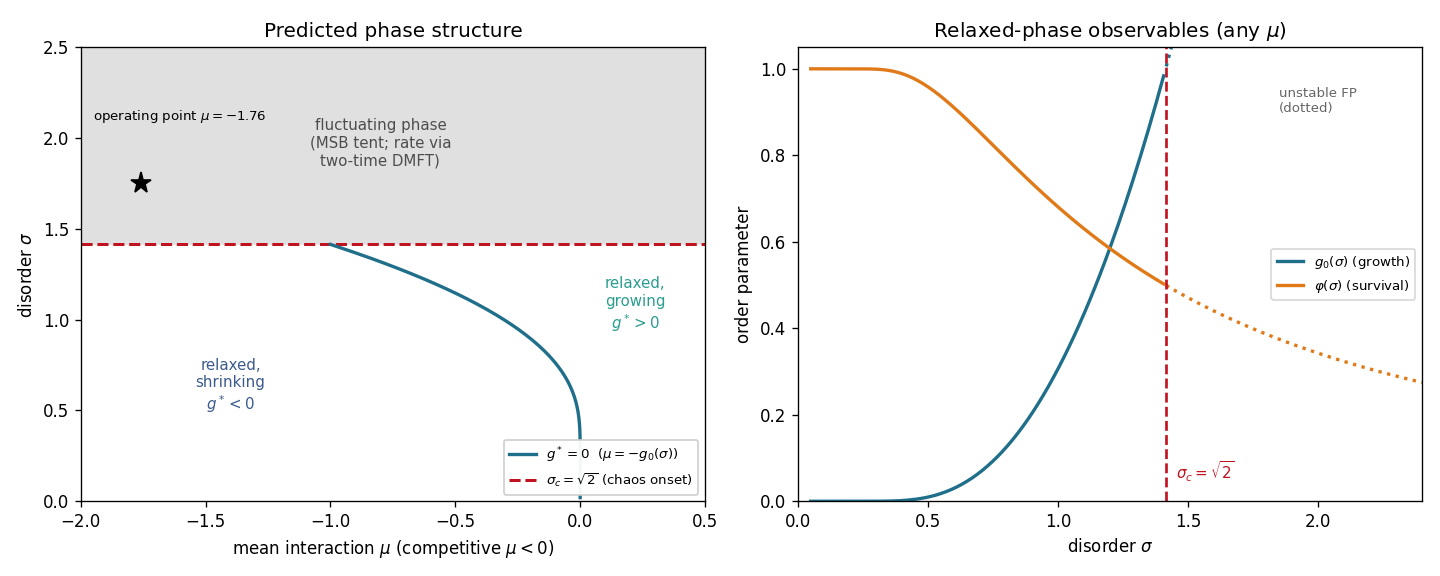
\includegraphics[width=\linewidth]{dmft_phase.png}
  \caption{Regular-graph theory at $\gamma=0$.  Left: the chaos onset $\sigma_c=\sqrt2$ is
  independent of $\mu$; the line $g^*=0$, $\mu=-g_0(\sigma)$, separates growing from shrinking
  relaxed economies.  The operating point lies in the fluctuating phase.  Right: the
  $\mu$-independent order parameters \eqref{eq:regular}; dotted where the fixed point is
  unstable.}
  \label{fig:phase}
\end{figure}

The theory was tested on the matching ensemble: a fully connected graph with
$W_{ij}=\mu/N+\sigma z_{ij}/\sqrt N$, $\gamma=0$, $N=1500$, $\lambda=0$ (Table~\ref{tab:regular},
Figure~\ref{fig:validation}).  Below $\sigma_c$ the growth rate and survival agree to one or two per
cent with nothing fitted.  The late-time fluctuation amplitude is below $0.005$ for $\sigma<\sqrt2$
and $0.038$, $0.13$, $0.21$ at $\sigma=1.6$, $2.0$, $2.5$.  And the $\mu$ independence holds: at
$\sigma=1$, $\mu=0,-1,-2$ give survival $0.688$, $0.687$, $0.685$ and growth rates $+0.317$,
$-0.682$, $-1.681$, shifted by $\mu$ to within $0.001$.

\begin{table}[htbp]
\centering\small
\begin{tabular}{rrrrrl}
\toprule
$\sigma$ & $g$ (sim) & $g^*$ (DMFT) & survival (sim) & $\varphi$ (DMFT) & phase\\
\midrule
0.40 & $-0.494$ & $-0.498$ & 0.991 & 0.989 & relaxed\\
0.70 & $-0.429$ & $-0.433$ & 0.860 & 0.854 & relaxed\\
1.00 & $-0.199$ & $-0.195$ & 0.690 & 0.681 & relaxed\\
1.20 & $+0.061$ & $+0.085$ & 0.601 & 0.585 & relaxed\\
1.35 & $+0.297$ & $+0.363$ & 0.540 & 0.523 & relaxed\\
1.60 & $+0.911$ & $+0.959$ & 0.371 & 0.440 & fluctuating\\
2.00 & $+2.032$ & $+2.272$ & 0.206 & 0.343 & fluctuating\\
2.50 & $+3.946$ & $+4.551$ & 0.090 & 0.261 & fluctuating\\
\bottomrule
\end{tabular}
\caption{Fully connected graph, $\mu=-0.5$, $\gamma=0$, $N=1500$.  Relaxed phase: mean
discrepancies $0.021$ in $g$ and $0.010$ in survival.  Beyond $\sigma_c$ the static solution
overshoots, since it is unstable there.}
\label{tab:regular}
\end{table}

\begin{figure}[htbp]
  \centering
  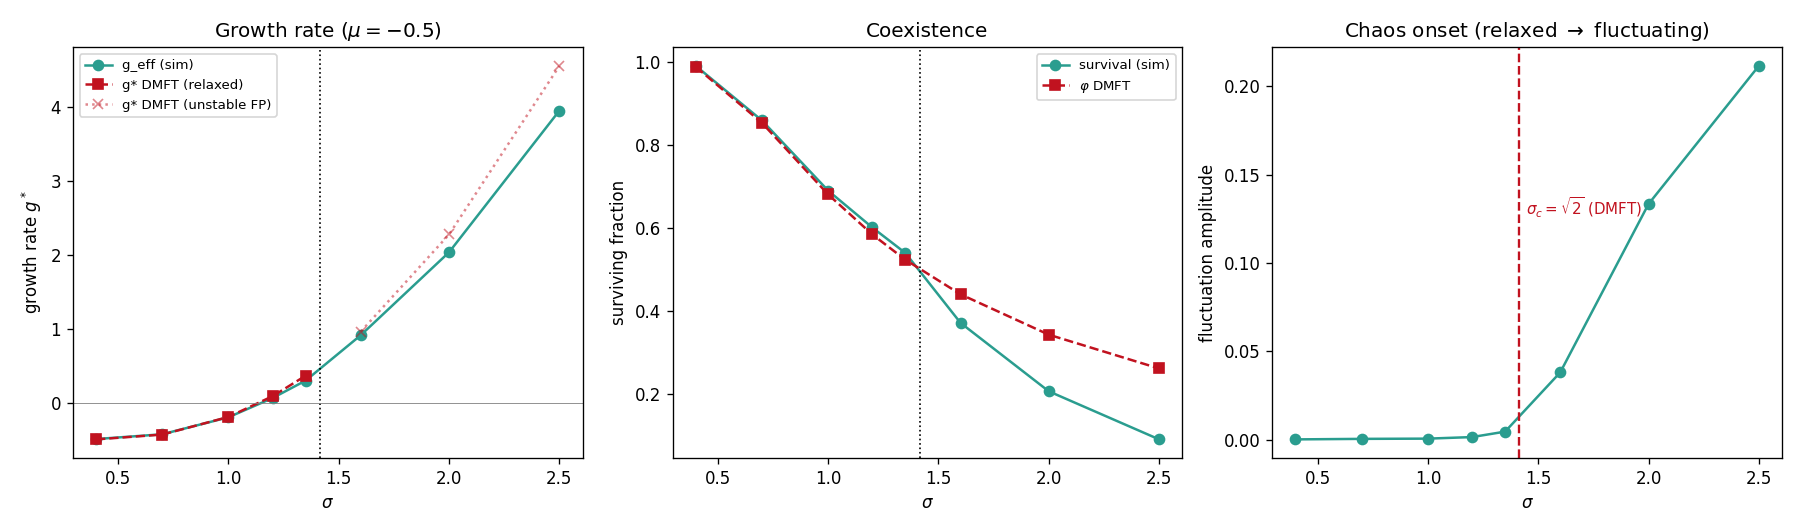
\includegraphics[width=\linewidth]{dmft_validation.png}
  \caption{Simulation (teal) against the DMFT (red) for Table~\ref{tab:regular}.  The fluctuation
  amplitude (right) switches on at the predicted $\sigma_c=\sqrt2$.}
  \label{fig:validation}
\end{figure}

\subsection{Power-law graphs: the stability line}
\label{sec:zerogrowth}

On a heterogeneous graph $B_p^*$ and $q_p^*$ vary with degree, so the mean interaction is no
longer a uniform shift, and the boundary becomes a curve $\sigma_c(\mu)$.  For the bilinear kernel
it can be written down exactly.

\begin{proposition}[Stability line, bilinear kernel; leading order]\label{prop:sigmac}
Let $K_{pr}=\rho_r\kappa_p\kappa_r$, $\lambda=0$, $\gamma=0$, and write averages over nodes as
$\langle\cdot\rangle$.  The fixed point loses stability at
\begin{equation}
  \sigma_c^{-2}=\bigl\langle\kappa^2\PhiN(\Delta_\kappa)\bigr\rangle,\qquad
  \Delta_\kappa=A\,\kappa^{-1/2}+M\,\kappa^{1/2},
  \label{eq:sigmac}
\end{equation}
where $A$ and $M$ solve
\begin{equation}
  \bigl\langle\kappa^2\Delta_\kappa\,w_1(\Delta_\kappa)\bigr\rangle=0,\qquad
  M=\mu\,\bigl\langle\kappa^{3/2}w_1(\Delta_\kappa)\bigr\rangle .
  \label{eq:sigmac-AM}
\end{equation}
To first order in the degree variance,
\begin{equation}
  \sigma_c(\mu)\simeq\sqrt2\left[1-\frac{\Var\kappa}{2}\left(1-\frac{\mu^2}{2\pi}\right)\right].
  \label{eq:sigmac-v}
\end{equation}
\end{proposition}
\begin{proof}
The closure factorises, $B_\kappa=\kappa\bar B$ and $q_\kappa=\kappa Q$, so
$\Delta_\kappa=(a+\mu\kappa\bar B)/(\sigma\sqrt{\kappa Q})$ has the stated form with
$A=a/\sigma\sqrt Q$ and $M=\mu\bar B/\sigma\sqrt Q$; the $\bar B$ equation gives the second relation
of \eqref{eq:sigmac-AM}.  The second-moment equation is $\sigma^2\langle\kappa^2w_2(\Delta_\kappa)\rangle=1$.
The stability operator $\sigma^2\varphi_pK_{pr}$ has rank one, with Perron root
$\sigma^2\langle\kappa^2w_0(\Delta_\kappa)\rangle$.  Equating the two and using $w_2-w_0=\Delta w_1$
gives the first relation.  For \eqref{eq:sigmac-v} write $\kappa=1+\epsilon$: at $\Var\kappa=0$,
$\Delta\equiv0$ and $M_0=\mu/\sqrt{2\pi}$; to second order in $\epsilon$,
$\Delta_\kappa\simeq\delta+M_0\epsilon-M_0\epsilon^2/2$ and $\Delta w_1(\Delta)\simeq\Delta/\sqrt{2\pi}+\Delta^2/2$.
The first relation fixes $\delta=-\Var\kappa\,(\tfrac32M_0+\sqrt{\pi/2}\,M_0^2)$, and then
$\langle\kappa^2\PhiN\rangle=\tfrac12[1+\Var\kappa\,(1-M_0^2)]$.
\end{proof}
On a regular graph $\Delta\equiv0$ and \eqref{eq:sigmac} reduces to $\sigma_c=\sqrt2$.  Degree
heterogeneity alone lowers the threshold, because hubs carry noise of amplitude $\propto\sqrt\kappa$.
A mean interaction of either sign raises it: a coherent fitness gradient across degree classes
spreads the $\Delta_\kappa$, and the threshold condition then forces their mean down, lowering the
weighted response.  Beyond first order the effect is asymmetric.  Competition loads the hubs and
removes the noisiest firms; mutualism favours them.  Table~\ref{tab:sigmac} compares the three
levels of description on the phase-grid graphs.  The exact relation \eqref{eq:sigmac} agrees with
the binned HDMFT to $0.002$ at $\alpha=6$ and to $0.03$ at $\alpha=3.5$ (the binning smooths the hub
tail).  At $\alpha=2.5$ the structural cutoff matters at weak competition and little at strong
competition.

\begin{table}[htbp]
\centering\small\setlength{\tabcolsep}{4pt}
\begin{tabular}{l|cccc|cccc|cccc}
\toprule
 & \multicolumn{4}{c|}{$\alpha=6$, $\Var\kappa=0.06$} & \multicolumn{4}{c|}{$\alpha=3.5$, $\Var\kappa=0.45$} & \multicolumn{4}{c}{$\alpha=2.5$, $\Var\kappa=2.4$}\\
$\mu$ & \eqref{eq:sigmac-v} & \eqref{eq:sigmac} & bil. & SCM & \eqref{eq:sigmac-v} & \eqref{eq:sigmac} & bil. & SCM & \eqref{eq:sigmac-v} & \eqref{eq:sigmac} & bil. & SCM\\
\midrule
$+1$ & 1.377 & 1.386 & 1.385 & 1.385 & 1.145 & 1.323 & 1.294 & 1.288 & -- & 0.997 & -- & 1.062\\
$0$  & 1.370 & 1.372 & 1.374 & 1.375 & 1.095 & 1.174 & 1.201 & 1.211 & -- & 0.767 & -- & 0.935\\
$-1$ & 1.377 & 1.383 & 1.384 & 1.384 & 1.145 & 1.288 & 1.286 & 1.290 & -- & 1.213 & -- & 1.222\\
$-2$ & 1.398 & 1.407 & 1.407 & 1.407 & 1.298 & 1.421 & 1.414 & 1.417 & -- & 1.480 & -- & 1.507\\
\bottomrule
\end{tabular}
\caption{Stability threshold at $\lambda=0$ on the phase-grid graphs ($N=4000$, $C=100$): first
order \eqref{eq:sigmac-v}, the exact bilinear relation \eqref{eq:sigmac} on the node degrees, and
the 60-class HDMFT with the bilinear and the SCM kernel.  The bilinear kernel is not a probability
at $\alpha=2.5$.  Source: \texttt{scripts/phase\_sigma\_c\_bilinear.py}.}
\label{tab:sigmac}
\end{table}

On the $\alpha=2.5$ phase-grid graph with the SCM kernel and $\lambda=10^{-3}$, the line rises
smoothly from $\sigma_c=0.94$ at $\mu=0$ to $1.63$ at $\mu=-2.5$; immigration raises it by about
$0.01$ everywhere.  (An earlier version of the solver evaluated the $\lambda>0$ Gaussian averages
with 80 Hermite nodes, which do not resolve the kink of \eqref{eq:immigration} over a width
$\sim\sqrt\lambda$; the stability radius then jumped between neighbouring $\sigma$.)

Figure~\ref{fig:phasetheory}b shows the stability lines for the whole family of graphs.  Heavier degree tails
lower $\sigma_c$ at weak competition ($0.79$ at $\alpha=2.2$ against $1.38$ at $\alpha=6$, $\mu=0$) and make
it rise faster with competition, so the lines cross near $\mu\simeq-1.5$ and the order is reversed at
strong competition ($1.71$ against $1.42$ at $\mu=-2.5$): competition removes the hubs, which are the
source of the instability.  The zero-growth line hardly depends on the topology (the four graphs
agree to $0.03$--$0.25$ in $\mu$ at every $\sigma$); what depends on it is how much of the line is
controlled, up to $\sigma\simeq1.33$ at $\alpha=6$ but only $0.81$ at $\alpha=2.2$.  At the operating point
every graph is above $\sigma_c$ and on the growing side of the line.

\begin{figure}[htbp]
  \centering
  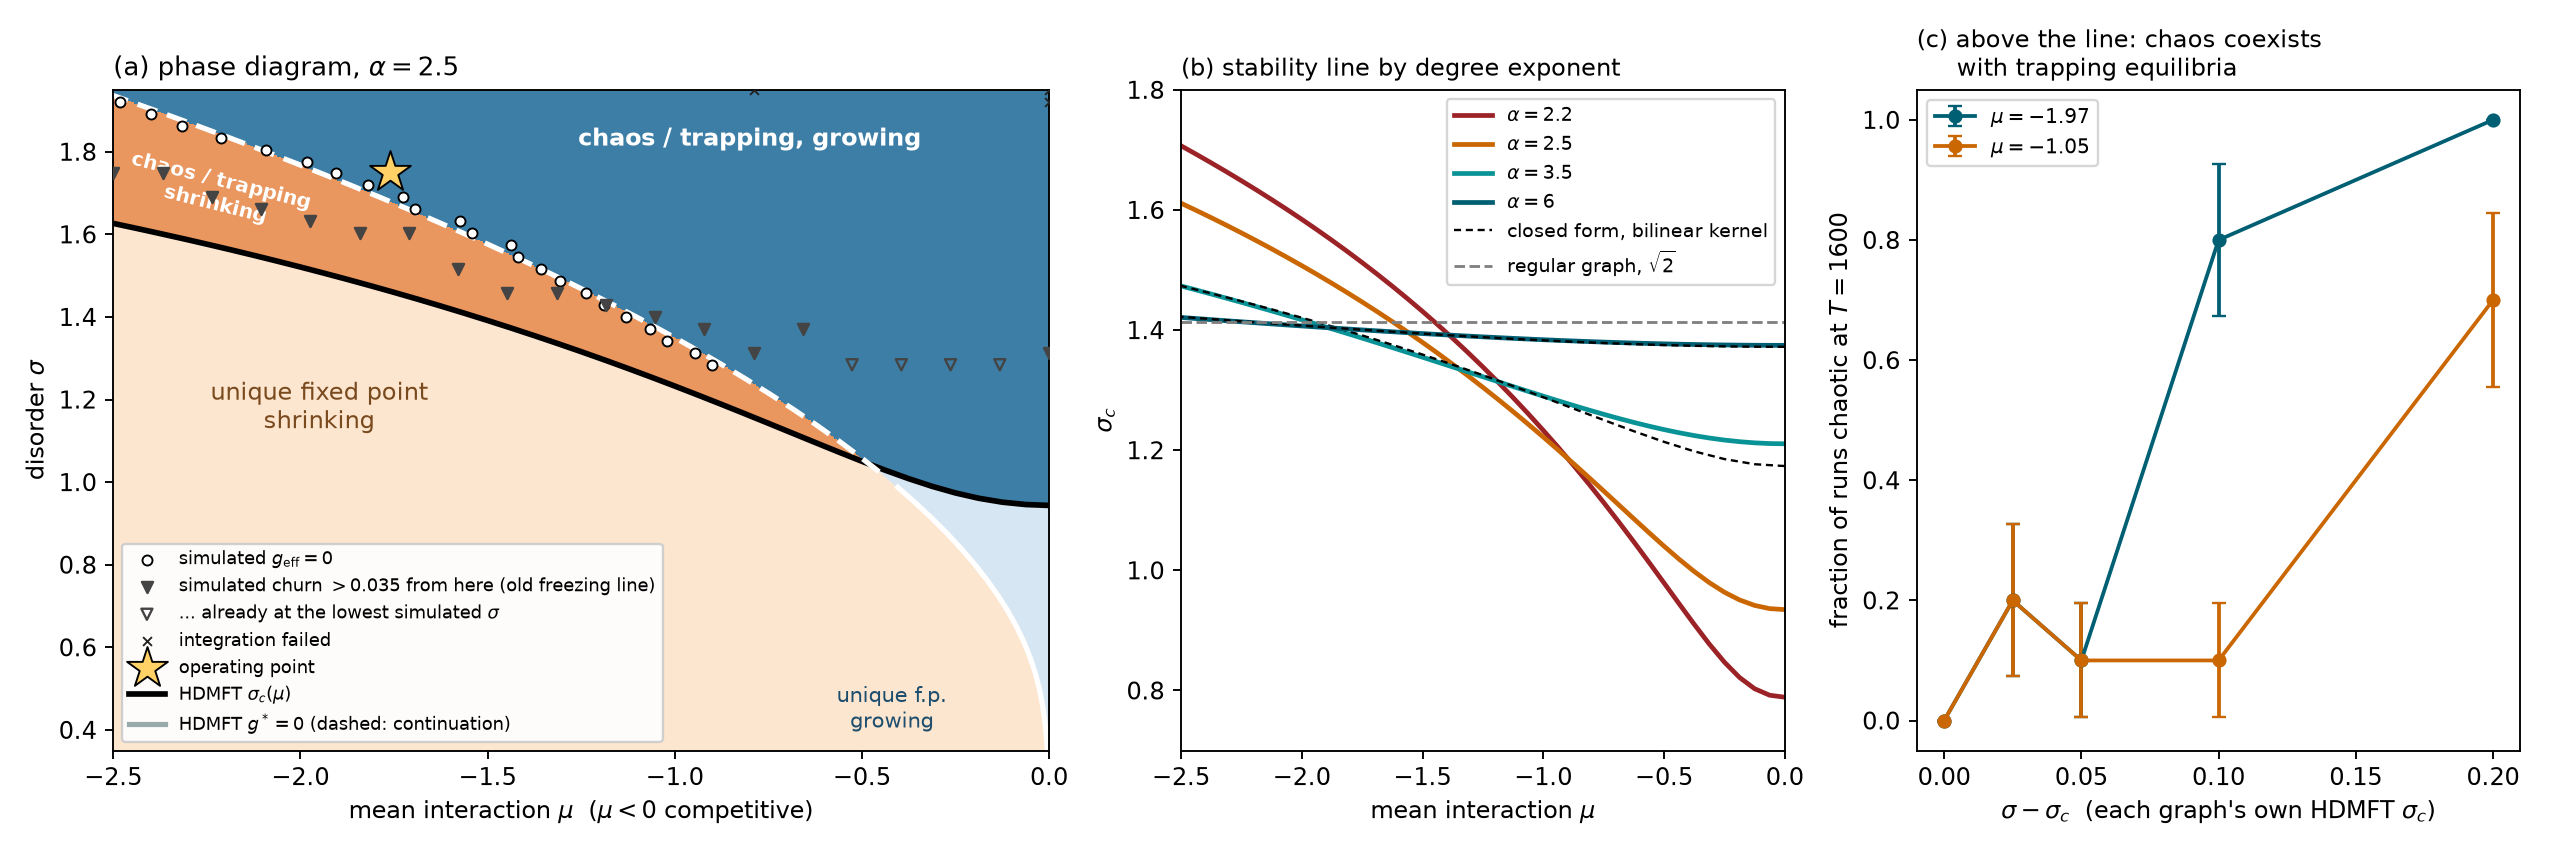
\includegraphics[width=\linewidth]{phase_theory.png}
  \caption{(a) Phase diagram for $\alpha=2.5$ ($N=4000$, $C=100$, $\lambda=10^{-3}$).  Regions
  from the HDMFT: below the stability line $\sigma_c(\mu)$ (black; 60 classes, SCM kernel) the
  composition has a unique fixed point; above it chaos coexists with trapping equilibria.  The
  zero-growth line (white; dashed where it continues an unstable fixed point) separates growing from
  shrinking economies.  Symbols are simulation: zero crossings of the growth rate, the $\sigma$ above
  which the median churn exceeds $0.035$ (the old freezing line; hollow where it is already exceeded
  at the lowest simulated $\sigma=1.28$), cells whose integration failed, and the operating point.
  (b) Stability line for $\alpha=2.2$--$6$ ($\lambda=0$) with the closed form for the bilinear kernel
  (dashed, where that kernel is a probability) and the regular-graph value $\sqrt2$.  (c) Fraction of
  runs chaotic at $T=1600$ against the distance from each graph's own $\sigma_c$, ten graphs per point.  Source: \texttt{scripts/plot\_phase\_theory.py}.}
  \label{fig:phasetheory}
\end{figure}

\paragraph{Zero growth.}
Since $g^*=1-a$, the zero-growth line is obtained by imposing $a=1$ and treating $\mu$ as the
unknown.  At fixed $\sigma$ the $2n+1$ unknowns $\{B_p^{(0)},q_p^{(0)}\}$ and $\mu^{(0)}$ solve
\begin{gather}
  B_p^{(0)}=\sum_rK_{pr}\,\sigma\sqrt{q_r^{(0)}}\,w_1(\Delta_r^{(0)}),\qquad
  q_p^{(0)}=\sum_rK_{pr}\,\sigma^2q_r^{(0)}\,w_2(\Delta_r^{(0)}),\nonumber\\
  1=\sum_p\rho_p\,\sigma\sqrt{q_p^{(0)}}\,w_1(\Delta_p^{(0)}),\qquad
  \Delta_p^{(0)}=\frac{1+\mu^{(0)}B_p^{(0)}}{\sigma\sqrt{q_p^{(0)}}} .
  \label{eq:zerogrowth}
\end{gather}
In the one-class limit this gives $\mu^{(0)}=-g_0(\sigma)$.  For the bilinear kernel the line solves
\[
  \sigma^2\langle\kappa^2w_2(\Delta_\kappa)\rangle=1,\qquad M=\mu\langle\kappa^{3/2}w_1(\Delta_\kappa)\rangle,\qquad
  A=\langle\kappa^{1/2}w_1(\Delta_\kappa)\rangle,
\]
the last being $a=1$ after the normalisation $\sigma\sqrt Q=1/\langle\kappa^{1/2}w_1\rangle$.  Expanding as for \eqref{eq:sigmac-v},
\begin{equation}
  \mu^{(0)}(\sigma)\simeq-g_0(\sigma)+c(\sigma)\,\Var\kappa,\qquad
  c(\sigma\to0)=0,\qquad c(\sigma\to\sqrt2)=\frac54-\frac\pi2\simeq-0.32,
  \label{eq:zg-v}
\end{equation}
with $c$ an explicit rational function of $\Delta$, $\PhiN(\Delta)$ and $\phiN(\Delta)$ at the regular
solution $\sigma^2w_2(\Delta)=1$ (\texttt{scripts/phase\_zero\_growth\_bilinear.py}; it matches the exact
bilinear line to $0.004$ at $\alpha=6$).  Heterogeneity moves the zero-growth line slightly towards
competition, so a heterogeneous economy grows a little faster at given $(\mu,\sigma)$.  The
coefficient is at most a third of that of $\sigma_c$ in \eqref{eq:sigmac-v}, which is why the zero-growth
lines of different graphs nearly coincide.  Each point must also be tested
against \eqref{eq:stability}: the solution is a controlled prediction only where the fixed point
is stable.

\begin{figure}[htbp]
  \centering
  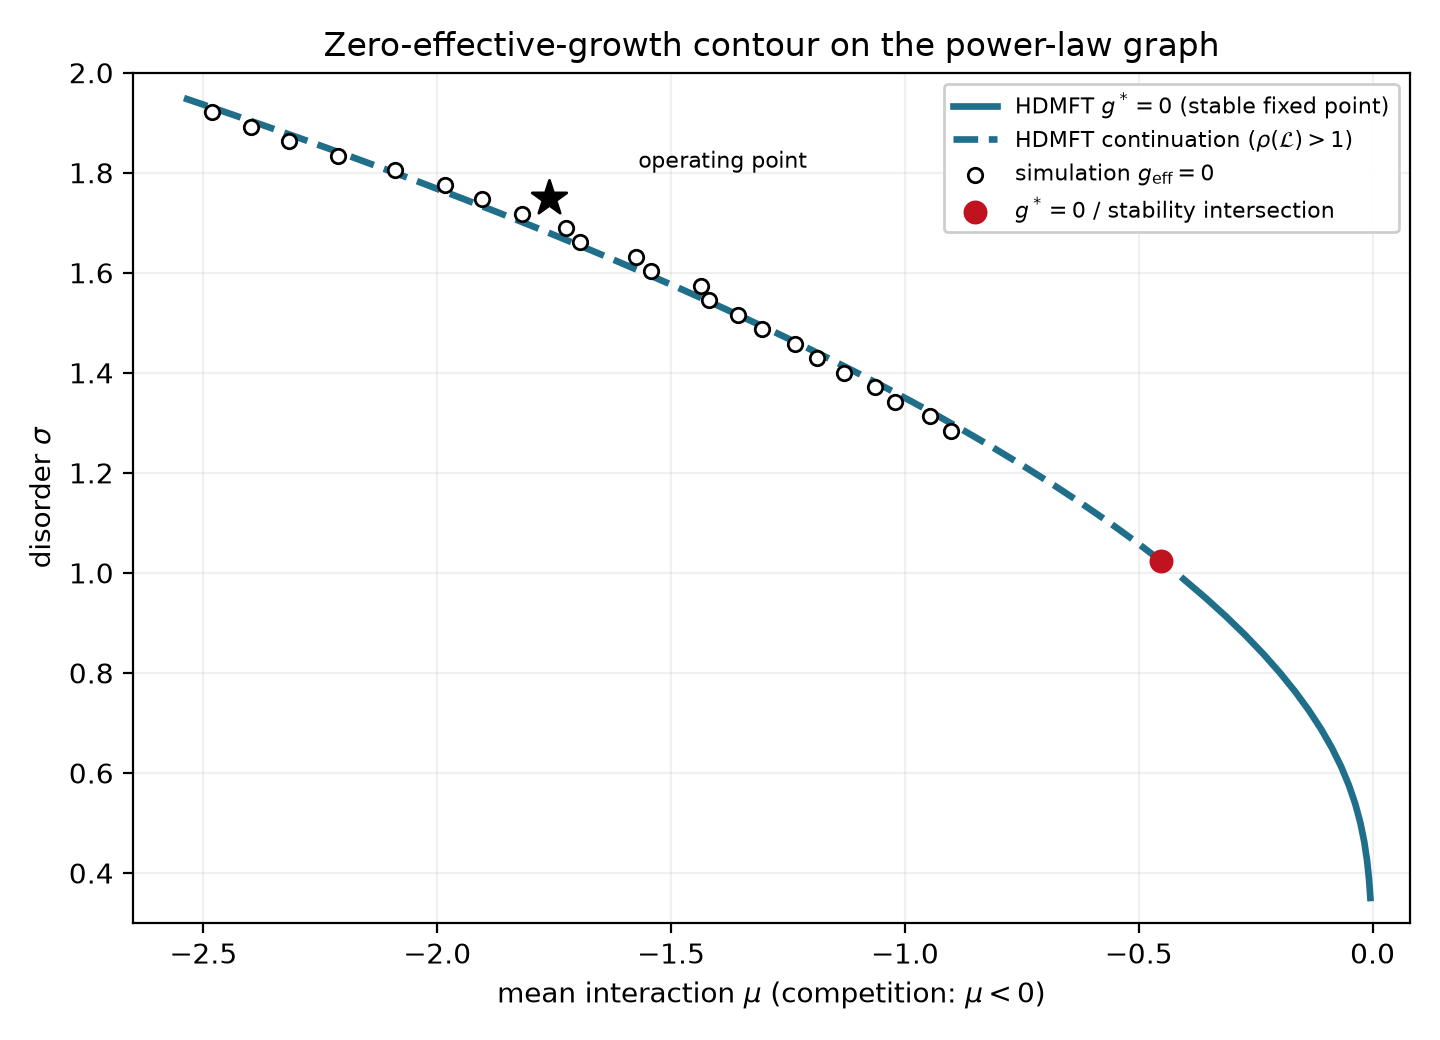
\includegraphics[width=0.8\textwidth]{zero_growth_line.png}
  \caption{HDMFT zero-growth line on a power-law graph ($N=4000$, target $C=100$, realised
  $81.998$, $\alpha=2.5$, 30 degree classes, SCM kernel) against the zero crossing of the median
  finite-time growth rate in simulation.  The star is the operating point.}
  \label{fig:zerogrowth}
\end{figure}

The line leaves the stable region at $(\mu,\sigma)=(-0.452,1.023)$, and every simulated point lies
above it (Figure~\ref{fig:zerogrowth}).  Its continuation through the unstable regime nonetheless
tracks the simulated contour with a mean absolute error of $0.029$ in $\mu$ over the 23 rows
with a sign change, and a mean bias of $0.003$.  At $\sigma=1.75$ it gives $\mu^{(0)}=-1.951$, so
the operating point $\mu=-1.76$ is predicted to grow, as it does.  Above $\sigma\simeq1.02$ this is
an empirically successful continuation, not a derivation: the controlled statement is
$\bar g=0$ computed with the two-time theory \eqref{eq:hdmft}.  Whether the agreement is exact
is open.

\subsection{Above the stability line}
\label{sec:above}

The simulated phase diagram classifies a cell as frozen when the late-time standard deviation of
the growth rates (the \emph{churn}) is below $0.035$.  Its freezing line lies $0.1$--$0.3$ above the
HDMFT $\sigma_c(\mu)$: $1.75$, $1.63$, $1.46$, $1.40$, $1.37$ against $1.63$, $1.52$, $1.38$, $1.25$,
$1.11$ at $\mu=-2.5$, $-1.97$, $-1.45$, $-1.05$, $-0.66$.  Three numerical checks on the same graph
ensemble locate the transition at the HDMFT line and explain the gap.
\begin{enumerate}
  \item \emph{Below $\sigma_c$ the fixed point is unique.}  Three initial conditions (one narrow,
        two broad log-normal) on the same graph and couplings freeze into the same state, to
        $10^{-4}$ in $\ln S$, up to the HDMFT $\sigma_c$ at every $\mu$ tested ($N=4000$).
  \item \emph{Above $\sigma_c$ frozen and chaotic runs coexist, at every $\mu$.}  For ten graphs
        per point, each with its own HDMFT $\sigma_c$ (which varies by $\pm0.015$ between graphs), the
        fluctuation amplitude (median time standard deviation of $\ln S$ of firms listed throughout)
        was measured in two windows, $[600,800]$ and $[1400,1600]$.  A run is frozen in both
        (amplitude $\lesssim10^{-3}$), still relaxing, or chaotic with the same amplitude in both:
        \begin{center}\small
        \begin{tabular}{l|ccccc}
        \toprule
        $\sigma-\sigma_c$ & $0$ & $0.025$ & $0.05$ & $0.10$ & $0.20$\\
        \midrule
        $\mu=-1.97$: frozen / relaxing / chaotic & 9/1/0 & 8/0/2 & 8/1/1 & 2/0/8 & 0/0/10\\
        $\mu=-1.05$: frozen / relaxing / chaotic & 9/1/0 & 8/0/2 & 9/0/1 & 9/0/1 & 2/1/7\\
        \bottomrule
        \end{tabular}
        \end{center}
        At $\sigma_c$ no run is chaotic.  Above it the chance of persistent chaos rises, steeply at
        strong competition (most graphs are chaotic by $\sigma_c+0.1$) and slowly at weak competition
        (by $\sigma_c+0.2$).  Frozen runs from different initial conditions end in different states,
        and one chaotic run was trapped between $T=800$ and $1600$.  This is the multiple-attractor
        regime of the disordered GLV beyond $\sigma_c$: the unique fixed point is gone, and a finite
        system can wander chaotically or be trapped by one of many stable equilibria, with a
        trapping probability that grows with the observation time.  A scan at $N=2000$, $4000$ and
        $8000$ (three graphs each, $\mu=-1.97$, $T=800$) shows no trend in $N$.
  \item \emph{The simulated line is a majority contour.}  It marks where most of the ten
        realisations of a cell fluctuate with churn above $0.035$; for example, the median churn at
        $\mu=-1.97$ crosses $0.035$ at $\sigma\simeq1.635$, the simulated line ($1.632$).  It is a
        statistic of the coexistence region at $N=4000$ and $T=400$, not a second transition.
\end{enumerate}
\paragraph{The ``divergent'' corner.}  At weak competition and strong disorder some grid runs fail to
integrate.  This is numerical, not a phase.  Integrated in chunks of $20$ time units with the state
clipped to $w\ge0$ between chunks, a failed run ($\sigma=1.95$, $\mu=-0.13$) reaches $T=400$ in about a
minute and stays bounded: $g\simeq6$--$60$, the largest firm has $S\simeq100$--$200$ (a share of
$2$--$5\%$), and only $120$--$300$ of the $4000$ firms are above the mean size at any time.  The grid
runs fail because the immigration floor, $w\simeq\lambda/N|f|\simeq5\times10^{-9}$ at $|f|\simeq50$, lies
far below the absolute tolerance $10^{-7}$ of the solver.  The corner is the strongly concentrated,
fast end of the fluctuating, growing phase, and the growth rate rises continuously into it.

The HDMFT stability line is therefore the phase boundary of the unique fixed point.  Above it
chaos coexists with trapping equilibria at every competition strength, and chaos takes over
within $0.1$ of the line at strong competition and within $0.2$ at weak competition.  Sources:
\texttt{scripts/phase\_attractors.py}, \texttt{scripts/phase\_coexistence.py},
\texttt{scripts/phase\_onset\_N.py}, \texttt{scripts/phase\_divergent\_check.py}.

%======================================================================
\section{The fluctuating phase: Gaussian fitness and one firm}
\label{sec:onefirm}

At the operating point the composition never settles.  Over a few hundred time units
$80$--$95\%$ of firms fall to the floor at least once and climb back: a node behaves as a niche
that successive firms occupy, with immigration as entry.  This section establishes that the
size--volatility statistics are those of a single firm \eqref{eq:firm} driven by the fitness law
of Proposition~\ref{prop:law}.

\subsection{Fitness statistics}
\label{sec:fitnesscheck}

Within a firm the measured fitness is $\Phi_i=\bPhi_i+f_i\eta_i(t)$ with $\eta_i$ of unit variance.
Its autocorrelation is smooth at short lags and well described by
$\rho(L)=(1+L/\tau)e^{-L/\tau}$ (Table~\ref{tab:fitness}).  The fitness law predicts each firm's
$(\bPhi_i,f_i)$ from its degree alone, given the order parameters.  Table~\ref{tab:cavity} uses the
order parameters measured as degree-weighted averages in the simulation.  Once its predicted mean
and spread are removed, the static field is a standard Gaussian to within an excess kurtosis of
$0.2$--$0.35$.  The amplitude is $\sigma\sqrt{\kappa(Q_0-Q_T)}$ to within $\pm13\%$, and the
extreme skew of $\bPhi$ on the $\alpha=2.5$ graph comes entirely from the mixture over degrees.

\begin{table}[htbp]
\centering\small\setlength{\tabcolsep}{4pt}
\begin{tabular}{lccccccc}
\toprule
graph, $\sigma$ & mean $\bPhi$ & sd $\bPhi$ & skew $\bPhi$ & $\bar f\pm{}$sd & corr$(\bPhi,f)$ & ACF $1/e$ & $\tau$\\
\midrule
$\alpha=6$, $1.75$   & $-0.95$ & $3.27$ & $-0.11$ & $1.82\pm0.41$ & $-0.09$ & $7.5$ & $3.51$\\
$\alpha=3.5$, $1.9$  & $-1.73$ & $3.70$ & $-0.87$ & $3.45\pm1.08$ & $-0.29$ & $3.5$ & $1.65$\\
$\alpha=2.5$, $1.75$ & $-0.97$ & $4.36$ & $-4.56$ & $2.12\pm1.15$ & $-0.42$ & $4.0$ & $1.89$\\
\bottomrule
\end{tabular}
\caption{Exact fitness of the full model, $N=8000$, $\lambda=10^{-3}$, eight economies, window
$[180,660]$.  On heavy tails hubs combine a large amplitude with a very negative mean.}
\label{tab:fitness}
\end{table}

\begin{table}[htbp]
\centering\footnotesize\setlength{\tabcolsep}{3pt}
\begin{tabular}{l|cccc|c|ccc}
\toprule
 & \multicolumn{4}{c|}{$(\bPhi-r_\kappa)/a_\kappa$} & $f/f_\kappa$ & sd $\bPhi$ & skew $\bPhi$ & corr$(\bPhi,f)$\\
graph, $\sigma$ & mean & sd & skew & exkurt & median (IQR) & \multicolumn{3}{c}{measured / law}\\
\midrule
$\alpha=6$, $1.75$   & $-0.003$ & $1.004$ & $-0.01$ & $0.23$ & $0.97$ ($0.87$--$1.09$) & $3.27/3.23$ & $-0.11/-0.09$ & $-0.09/-0.12$\\
$\alpha=3.5$, $1.9$  & $0.006$  & $1.006$ & $-0.02$ & $0.28$ & $0.98$ ($0.88$--$1.09$) & $3.69/3.67$ & $-0.87/-0.87$ & $-0.29/-0.33$\\
$\alpha=2.5$, $1.75$ & $0.004$  & $0.997$ & $-0.03$ & $0.35$ & $0.96$ ($0.83$--$1.12$) & $4.36/4.25$ & $-4.56/-4.47$ & $-0.42/-0.41$\\
\bottomrule
\end{tabular}
\caption{Cavity check of Proposition~\ref{prop:law}, firm by firm.}
\label{tab:cavity}
\end{table}

\begin{figure}[htbp]
  \centering
  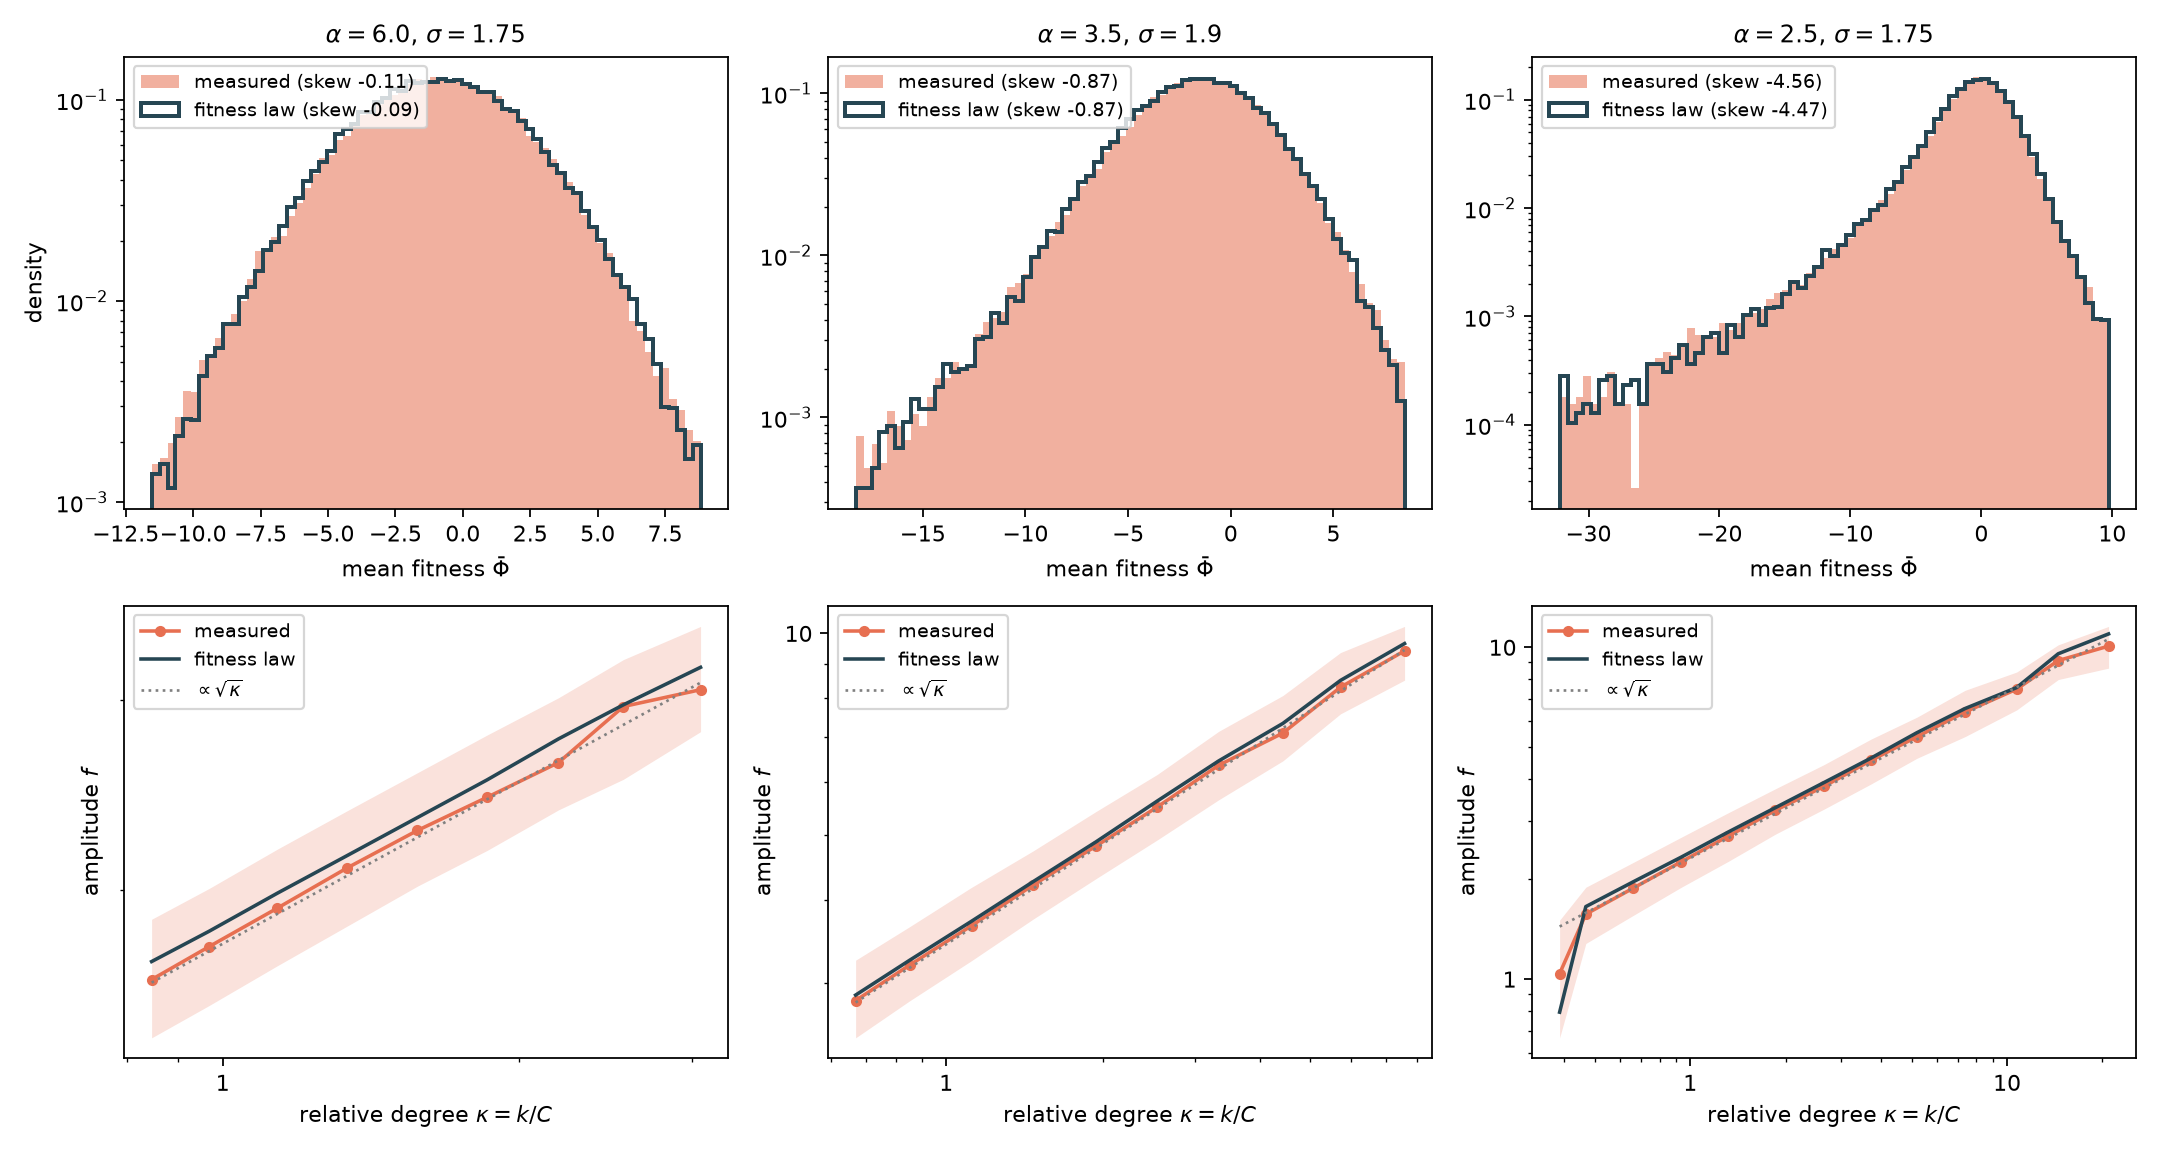
\includegraphics[width=\linewidth]{fitness_law.png}
  \caption{The fitness law against the full model ($N=8000$, $\lambda=10^{-3}$, eight economies).  Top:
  per-firm mean fitness, measured and sampled from Proposition~\ref{prop:law} with the simulation's
  order parameters; the left skew on heavy tails comes from the mixture over degrees.  Bottom:
  amplitude $f$ against relative degree (median and quartiles), with the law $f_\kappa\propto\sqrt\kappa$.
  Source: \texttt{scripts/lifecycle/plot\_fitness\_law.py}.}
  \label{fig:fitnesslaw}
\end{figure}

The fraction of time listed follows consequence~3 in its degree dependence (at $\alpha=2.5$ it
falls from $0.57$ to $0.30$ across the degree range, against $0.50$ to $0.31$) and sits
$0.04$--$0.07$ above it, because a firm stays listed for a while as it decays after its fitness
turns negative.

\subsection{Single-firm reduction}
\label{sec:reduction}

Replace the network by independent copies of \eqref{eq:firm} with $\Phi_i=\bPhi_i+f_i\eta_i$, where
$(\bPhi_i,f_i)$ are each firm's measured values and $\eta_i$ is a Gaussian process with the fitted
$\rho$, and apply the same estimators.  The two panels used here are defined in
Section~\ref{sec:panels}; for now it is enough that they count different firms.

\begin{table}[htbp]
\centering\small\setlength{\tabcolsep}{4pt}
\begin{tabular}{ll|cc|cc}
\toprule
 & & \multicolumn{2}{c|}{full model} & \multicolumn{2}{c}{single-firm surrogate}\\
graph & panel & $\beta$ & $\zeta_q/\zeta_1$, $q=2,3,4$ & $\beta$ & $\zeta_q/\zeta_1$\\
\midrule
$\alpha=6$, $\sigma=1.75$   & survivor & $0.894$ & $1.96,\,2.87,\,3.70$ & $0.862$ & $1.95,\,2.82,\,3.62$\\
                            & spells   & $0.554$ & $1.84,\,2.50,\,3.00$ & $0.536$ & $1.77,\,2.33,\,2.74$\\
$\alpha=3.5$, $\sigma=1.9$  & spells   & $0.284$ & $1.79,\,2.30,\,2.53$ & $0.288$ & $1.79,\,2.37,\,2.76$\\
$\alpha=2.5$, $\sigma=1.75$ & survivor & $0.414$ & $1.87,\,2.58,\,3.15$ & $0.474$ & $1.87,\,2.60,\,3.21$\\
                            & spells   & $0.191$ & $1.42,\,1.34,\,0.95$ & $0.183$ & $1.49,\,1.61,\,1.52$\\
\bottomrule
\end{tabular}
\caption{The surrogate against the full model ($T=480$ for spells).  Spell rows use the fixed-range
estimator of Section~\ref{sec:data}; survivor rows use the peak-start fit of the original analysis.
Data: $\beta\approx0.20$, ratios $2.0,\,2.6,\,2.9$.  Source: \texttt{scripts/lifecycle/recompute\_tables.py}.}
\label{tab:surrogate}
\end{table}

\begin{proposition}[Single-firm reduction; numerical]\label{prop:reduction}
Under both panels, $\beta$ and the ratio curve are properties of the one-firm process
\eqref{eq:firm} driven by a Gaussian fitness.  The graph enters only through the joint law of
$(\bPhi,f)$ and the correlation time.
\end{proposition}
On the spell panel the agreement is within $0.02$ in $\beta$ and $0.25$ in the ratios, except at
$q=3$, $4$ on the flattest heavy-tail curve, where the full model bends further; on the survivor
panel it is within $0.06$ in $\beta$ (Table~\ref{tab:surrogate}).  This is what the cavity picture predicts at
leading order, where the field on a firm is Gaussian and independent of the firm's own size.  It
also settles where $\beta$ comes from: a single firm in a Gaussian field contains no cross-firm
correlation, so the size--volatility law is a property of the one-firm dynamics and of the
distribution of fitness across firms.

\subsection{Solving the two-time theory}
\label{sec:twotime}

The order parameters can be computed without simulation by solving \eqref{eq:hdmft} forward in
time: each degree class runs \eqref{eq:firm} for a few hundred paths in a Gaussian field whose
covariance is updated from the paths until it is self-consistent.  We use 25--50 classes from
the realised degree sequence and the SCM kernel.  The solver converges for $\alpha\ge2.5$.  At
$\alpha=2.2$ it does not (relative error $15$--$18\%$ at twice the iterations, $g$ still
drifting): there the field is carried by about four neighbours (Section~\ref{sec:finiteC}) and is
not Gaussian, so the cavity step itself fails.

%======================================================================
\section{Which firms are counted}
\label{sec:panels}

\subsection{Two panels}

Moran, Secchi and Bouchaud use an unbalanced panel \citep{moran2024}: every Compustat firm with at
least two annual growth rates contributes, over its own listed life, a volatility
$v_i=\sqrt{\pi/2}\,T_i^{-1}\sum_t|g_{it}-\bar g_i|$ and a size equal to its lifetime mean.  Two
estimators are applied to the model.
\begin{itemize}
  \item The \emph{survivor} (balanced) panel keeps only firms whose share stays above $10^{-6}$
        throughout a window of length $T$.  It counts firms on their plateau.
  \item The \emph{spell} (unbalanced) panel follows the empirical protocol.  A spell is a maximal
        stretch with $S>\Sthr=8\lambda$ (the share $10^{-6}$ at $\lambda=10^{-3}$, $N=8000$), and
        each spell counts as one firm.  It counts entries, plateaux and exits.
\end{itemize}
The survivor panel has no long-window limit: its survivors are firms that did not dip during
$T$, and their number vanishes as $T\to\infty$.  At $\alpha=2.5$ its $\beta$ drifts from $0.414$ to
$0.354$ between $T=60$ and $480$.  Only spells cut by the window edges depend on $T$ in the spell
panel, and its $\beta$ converges: $0.110$, $0.081$, $0.084$, $0.080$ for $T=240$--$1920$ at
$\alpha=2.2$, and $0.461$, $0.422$, $0.391$, $0.374$ at $\alpha=6$ (peak-start fit), with the cut-off
share falling to $3$--$4\%$ (the slow approach is explained in Section~\ref{sec:rice}).  The spell panel is
therefore the model counterpart of the data, and Section~\ref{sec:spells} treats it.  The survivor
panel isolates the plateau fluctuations, which are the large-firm limit of every spell; its
theory (the adiabatic law, an exact sum rule and the degree channel) is in
Appendices~\ref{sec:adiabatic} and \ref{sec:survivor}.

\subsection{A general multiscaling criterion}
\label{sec:criterion}

Both panels write the volatility as a deterministic function of size times a random factor.

\begin{proposition}[Multiscaling criterion]\label{prop:criterion}
Let $v=A(\bar S)\,X$ with $X$ random given $\bar S$, and let $c_n(\bar S)$ be the cumulants of $\ln X$
given $\bar S$, so that $s^2=c_2=\Var(\ln X\mid\bar S)$.  Then, exactly,
\begin{equation}
  \zeta_q-q\,\zeta_1=-\sum_{n\ge2}\frac{q^n-q}{n!}\,\frac{dc_n}{d\ln\bar S}
  =-\frac{q(q-1)}{2}\,\frac{ds^2}{d\ln\bar S}-\frac{q^3-q}{6}\,\frac{dc_3}{d\ln\bar S}-\dots,
  \label{eq:criterion}
\end{equation}
so at second-cumulant order the ratio curve bends below $q$ if and only if the conditional
log-variance of $X$ grows with size.
\end{proposition}
\begin{proof}
$\zeta_q=q\beta_A-d\ln\E[X^q\mid\bar S]/d\ln\bar S$ with $\ln\E[X^q\mid\bar S]=\sum_nq^nc_n/n!$.
Subtract $q$ times the case $q=1$; the $n=1$ terms cancel.
\end{proof}
A fixed-shape law has $s^2$ constant and $\zeta_q=q\zeta_1$.  Multiscaling needs a random factor
whose spread opens up with size.  On the survivor panel $X=\sqrt\kappa$; on the spell panel
$X=\ell/n$, a log range over a lifetime.  At second-cumulant order \eqref{eq:criterion} bends the curve as $q(q-1)$, which cannot produce a
hard saturation of the ratio curve; that would need higher cumulants.

%======================================================================
\section{The spell panel: life cycles}
\label{sec:spells}

Under the empirical protocol a firm is counted from entry to exit, and its volatility includes
the rise from the listing threshold and the fall back to it.

\subsection{The lifetime identity}
\label{sec:identity}

\begin{proposition}[Lifetime identity; exact]\label{prop:identity}
Let a spell start and end at $\Sthr$, with $n$ growth steps $g_t=\Delta\ln S$.  Then $\bar g=0$ and
\begin{equation}
  v=\sqrt{\tfrac\pi2}\;\frac{2\ell+V_p}{n},\qquad\ell=\ln\frac{S_{\max}}{\Sthr},
  \label{eq:identity}
\end{equation}
where $V_p\ge0$ is the total variation in excess of one rise and one fall.  For any firm, with
entry size $S_a$ and exit size $S_b$,
\begin{equation}
  v\ge\sqrt{\tfrac\pi2}\;\frac{2\ln\bigl(S_{\max}/\max(S_a,S_b)\bigr)}{n}.
  \label{eq:bound}
\end{equation}
\end{proposition}
\begin{proof}
Split the steps at the peak into a set $A$ (a fraction $x$ of the steps) and $B$.  With
$R_a=\ln(S_{\max}/S_a)$, $R_b=\ln(S_{\max}/S_b)$ and $\bar g=(R_a-R_b)/n$,
$\sum_t|g_t-\bar g|\ge|\sum_A(g_t-\bar g)|+|\sum_B(g_t-\bar g)|=2[(1-x)R_a+xR_b]\ge2\min(R_a,R_b)$.  For
a complete spell $R_a=R_b=\ell$, and the bound is the rise-and-fall part of the total variation.
\end{proof}
The bound \eqref{eq:bound} is model-free and can be evaluated firm by firm in data.  In the
surrogate at $\alpha=6$, \eqref{eq:identity} holds to a median relative error of
$2.5\times10^{-3}$ on the $87\%$ of spells complete at $T=480$, and the rise-and-fall term carries
$100\%$, $95\%$ and $74\%$ of $v$ at the low end, middle and top of the decline branch.  Under the
unbalanced panel a firm's volatility is essentially its log range over its lifetime; plateau
fluctuations matter only for the largest firms.  The survivor panel is the opposite limit: its
firms never rise or fall.

\subsection{Spells are humps}
\label{sec:humps}

The plateau term $V_p$ is smaller than the adiabatic law suggests.  In the single-firm process
with the $\alpha=6$ fitness, complete decline-branch spells shorter than about $8\tau$ (three
quarters of them) have total variation $2\ell$ to within the discretisation of the first and last
step: a spell is a single hump in $\ln S$, rising out of the threshold and falling back.  Its flanks
are the parabolae of \eqref{eq:mills}, and a parabolic hump,
$\ln S=\ln S_{\max}-t^2/2w^2$ above $\Sthr$, has
\begin{equation}
  \ln\frac{S_{\max}}{\bar S}=\frac12\ln\frac{4\ell}{\pi},
  \label{eq:hump}
\end{equation}
about $1.0$ for $\ell\approx6$, against a measured median of $0.96$--$1.0$ at every spell length.  Adding
the adiabatic plateau volatility $\sqrt D/\bar S$ to the life-cycle term double-counts the hump and
overshoots $v$ by a factor of about $1.5$.  Longer spells are $K$ humps merged by $K-1$ dips that
did not kill: each merge adds about $(0.35$--$0.4)\times2\ell$ to the total variation, and the length
grows by about $4.3\tau$ per hump.  The resulting hump law,
$v\simeq\sqrt{\pi/2}\,[\text{range}+2\delta\ell(K-1)]/n$ with $\delta\simeq0.35$, gives the volatility
of each spell to $4$--$10\%$, so the volatility of a spell is set by the same dip statistics as its
lifetime.  It does not yet give the exponents: they come out about $0.08$ too high at every $q$,
because the largest firms carry extra variation from fitness fluctuations that never reach zero.
The spell exponents quoted below are therefore those of the single-firm process
(Proposition~\ref{prop:reduction}), computed numerically; the hump picture explains their structure.
Source: \texttt{scripts/lifecycle/spell\_anatomy\_merges.py}.

\subsection{Exponents of the life-cycle part}

Write the rise-and-fall part as $v_{\rm tr}=c\,\ell/n$, $c=2\sqrt{\pi/2}$.  If $\ell$ and $n$ are
independent at fixed $\bar S$ and $S_{\max}\propto\bar S$,
\begin{equation}
  \zeta_q^{\rm tr}\simeq\zeta_q[n^{-1}]-\frac{d\ln\E[\ell^q\mid\bar S]}{d\ln\bar S}
  \simeq\zeta_q[n^{-1}]-\frac q\ell ,
  \label{eq:lifetimerep}
\end{equation}
where $\zeta_q[n^{-1}]$ are the exponents of the inverse lifetime.  The life-cycle exponent is a
lifetime--size exponent lowered by a logarithmic correction set by the depth of entry.

\begin{table}[htbp]
\centering\footnotesize\setlength{\tabcolsep}{2.5pt}
\begin{tabular}{c|cc|c|c|c|c}
\toprule
$\lambda$ & $\ell$ & $\frac{d\ln\ell}{d\ln S}$ ($1/\ell$) & $\zeta_q^{\rm tr}$ & r.h.s.\ of \eqref{eq:lifetimerep} & $\zeta_q[n^{-1}]$ & $\zeta_q/\zeta_1$ of $v$\\
\midrule
$10^{-4}$ & $8.3$ & $0.089$ ($0.121$) & $.444,\,.748,\,.969,\,1.14$ & $.445,\,.749,\,.973,\,1.15$ & $.534,\,.927,\,1.24,\,1.51$ & $1.87,\,2.59,\,3.17$\\
$10^{-3}$ & $6.0$ & $0.132$ ($0.167$) & $.521,\,.885,\,1.16,\,1.39$ & $.520,\,.883,\,1.16,\,1.39$ & $.652,\,1.15,\,1.56,\,1.91$ & $1.90,\,2.67,\,3.32$\\
$10^{-2}$ & $3.7$ & $0.241$ ($0.269$) & $.611,\,1.05,\,1.39,\,1.67$ & $.610,\,1.04,\,1.37,\,1.65$ & $.850,\,1.52,\,2.10,\,2.62$ & $1.93,\,2.77,\,3.50$\\
\bottomrule
\end{tabular}
\caption{Complete spells on the decline branch; surrogate with the $\alpha=6$ fitness, $T=480$,
$q=1,\dots,4$, fixed-range bins.  Eq.~\eqref{eq:lifetimerep} holds for the life-cycle part to $0.02$.}
\label{tab:lifetime}
\end{table}

Equation~\eqref{eq:lifetimerep} is exact for $v_{\rm tr}$ to within $0.02$
(Table~\ref{tab:lifetime}), but $v$ also contains the plateau part, which dilutes the bend.  At
$\lambda=10^{-3}$ the full volatility of complete spells has $\zeta_q=0.396$, $0.751$, $1.06$, $1.32$,
against $0.521$, $0.885$, $1.16$, $1.39$ for $v_{\rm tr}$: the life-cycle part alone bends the ratio
curve two to three times as strongly as $v$ does.  The life cycle is the mechanism, but a quantitative spell
theory must combine it with the plateau law of Section~\ref{sec:adiabatic}, and the two are not
additive (Section~\ref{sec:open}).

\subsection{Why the ratio curve bends}

By Proposition~\ref{prop:criterion} with $X=\ell/n$, the relevant spread is that of $\ln n$.  At
$\alpha=6$ ($\lambda=10^{-3}$), $\Var(\ln n\mid\bar S)$ rises from $0.29$ to $0.65$ across the larger
half of spells while the mean lifetime grows from $21$ to $86$.  The measured bend of the lifetime
exponents, $\zeta_q[n^{-1}]-q\zeta_1[n^{-1}]=0$, $-0.16$, $-0.40$, $-0.70$, has the predicted sign;
the second-cumulant estimate ($0$, $-0.23$, $-0.68$, $-1.35$) is close at $q=2$ and overshoots at
higher $q$, as an expansion in $q^2$ must.

The mechanism is a crossover between two kinds of exit.  A small firm lives through a single
positive excursion of its fitness, and such excursions have fairly regular lengths.  A large firm
exits only on a rare deep dip, a nearly memoryless event, so its lifetime is close to
exponential, for which $\Var\ln n=\pi^2/6\approx1.64$.  The spread grows with size until exits
are memoryless and then saturates.  Like the degree channel, the life-cycle bend is a crossover,
not an asymptotic law.

\subsection{The lifetime law}
\label{sec:rice}

\paragraph{Exact solution of the one-firm equation.}  At $\lambda=0$, \eqref{eq:firm} is linear in
$1/S$: $d(1/S)/dt=-\Phi/S+1$.  With the integrated fitness $\mathcal A(t)=\int^t\Phi$,
\begin{equation}
  \frac1{S(t)}=\int_{-\infty}^t e^{-[\mathcal A(t)-\mathcal A(t')]}\,dt' .
  \label{eq:exact}
\end{equation}
The size is a soft minimum over the drawdowns of the integrated fitness.  Near a downcrossing of
$\Phi$ with slope $-s$, $\Phi\simeq-s(t-t_0)$, \eqref{eq:exact} gives the inverse Mills ratio,
\begin{equation}
  S(t)=\sqrt s\,\frac{\phiN(\theta)}{\PhiN(-\theta)}\Big|_{\theta=\sqrt s\,(t-t_0)}\!\!,\qquad
  S(t_0)=\sqrt{2s/\pi},\qquad
  S(t)\simeq\sqrt{\tfrac{s}{2\pi}}\;e^{-[\mathcal A(t_0)-\mathcal A(t)]}\quad(\theta\gg1):
  \label{eq:mills}
\end{equation}
the firm tracks its fitness until the crossing, and then decays by the area of the dip, with a
prefactor fixed by the crossing slope.  Near the floor, with $S\ll\Phi$, the immigration term
gives the mirror image, $S(t)\simeq\lambda\int^te^{\mathcal A(t)-\mathcal A(t')}dt'$.

\paragraph{Kill and entry rules.}  A spell therefore ends at the first negative excursion of $\Phi$
whose area exceeds
\begin{equation}
  \ell_c(s)=\ln\frac{\sqrt{s/2\pi}}{\Sthr},
  \label{eq:kill}
\end{equation}
and a firm at the floor lists once $\mathcal A$ has risen by $\ell_e(s)=\ln\bigl(\Sthr\sqrt{s/2\pi}/\lambda\bigr)$
since the upcrossing.  Both thresholds are explicit and contain no fitted constant.  In the
one-firm process with the $\alpha=6$ fitness ($f=1.82$, $\tau=3.51$, $\lambda=10^{-3}$), the kill rule
classifies $96$--$98\%$ of the dips of listed firms correctly at every $u$, and the empirical
threshold sits at area $=\ell_c$.  The errors are dips that begin before $S$ has recovered from
the previous one, where \eqref{eq:mills} overestimates $S(t_0)$.  Applied to the Gaussian
fitness path alone, the two rules reproduce the spell lifetimes above their lower quartile to
$5$--$10\%$; they miss only the $4$--$9\%$ of spells shorter than four time units, in which the
firm never reaches its fitness.

\paragraph{Mean lifetime.}  The spell lifetime is thus a functional of a Gaussian process.  Kills
occur at Rice's downcrossing rate $\nu(u)=e^{-u^2/2}/(2\pi\tau)$, $u=\bPhi/f$, thinned by the
probability that a dip kills, so
\begin{equation}
  \bar L(u)=\frac{\PhiN(u)}{\nu(u)\,P_{\rm kill}(u)},\qquad
  P_{\rm kill}(u)=\Pr\bigl[\text{dip area}>\ell_c(f\dot s)\bigm|\text{downcrossing of }{-u}\bigr].
  \label{eq:lifetime}
\end{equation}
$P_{\rm kill}$ is a level-crossing statistic, computed from the Slepian model: $\eta$
conditioned on $\eta(0)=-u$ and $\eta'(0)=-\dot s$, with $\dot s$ drawn from the Rayleigh law of
crossing slopes.  Rice excursions merge into one spell by the factor $1/P_{\rm kill}$, which is not a constant: it
grows from $1.5$ at $u=-0.5$ to $5$ at $u=2$.  For $u\gg1$ dips are short parabolae,
$\Phi\simeq f[ut^2/2\tau^2-\dot st]$, of area $\tfrac23f\dot s^3\tau^4/u^2$, and
\begin{equation}
  -\ln P_{\rm kill}\simeq\frac12\left(\frac{3\,\ell_c}{2f\tau}\right)^{2/3}u^{4/3},\qquad
  \ln\bar L\simeq\frac{u^2}2+\frac12\left(\frac{3\,\ell_c}{2f\tau}\right)^{2/3}u^{4/3}+\ln(2\pi\tau) .
  \label{eq:largeu}
\end{equation}

\begin{table}[htbp]
\centering\small\setlength{\tabcolsep}{4pt}
\begin{tabular}{c|ccc|cc|c}
\toprule
$u$ & $P_{\rm kill}$ ODE & Slepian & \eqref{eq:largeu} & $\bar L$ ODE & $\bar L$ \eqref{eq:lifetime} & $\Var\ln L$ ODE\\
\midrule
$-0.5$ & $0.719$ & $0.669$ & -- & $14.9$ & $11.5$ & $0.81$\\
$0$    & $0.626$ & $0.575$ & -- & $22.7$ & $19.2$ & $0.92$\\
$0.5$  & $0.511$ & $0.475$ & $0.846$ & $40.2$ & $36.4$ & $1.08$\\
$1.0$  & $0.390$ & $0.374$ & $0.642$ & $83.2$ & $81.8$ & $1.33$\\
$1.5$  & $0.294$ & $0.284$ & $0.458$ & $221.5$ & $223$ & $1.63$\\
$2.0$  & $0.214$ & $0.207$ & $0.312$ & $(645)$ & $769$ & $(1.81)$\\
$3.0$  & $0.116$ & $0.098$ & $0.128$ & -- & -- & --\\
$5.0$  & -- & $0.015$ & $0.015$ & -- & -- & --\\
\bottomrule
\end{tabular}
\caption{Lifetime law of the one-firm process, $\alpha=6$ fitness.  ODE: $300$ firms over
$T=1500$ ($120$ over $T=6000$ for $u\ge1.5$); bracketed values are biased by spells as long as the
run.  The column \eqref{eq:lifetime} uses the Slepian $P_{\rm kill}$ and $\PhiN(u)$ and no
simulation.  Source: \texttt{scripts/lifecycle/kill\_rule.py}.}
\label{tab:rice}
\end{table}

\begin{figure}[htbp]
  \centering
  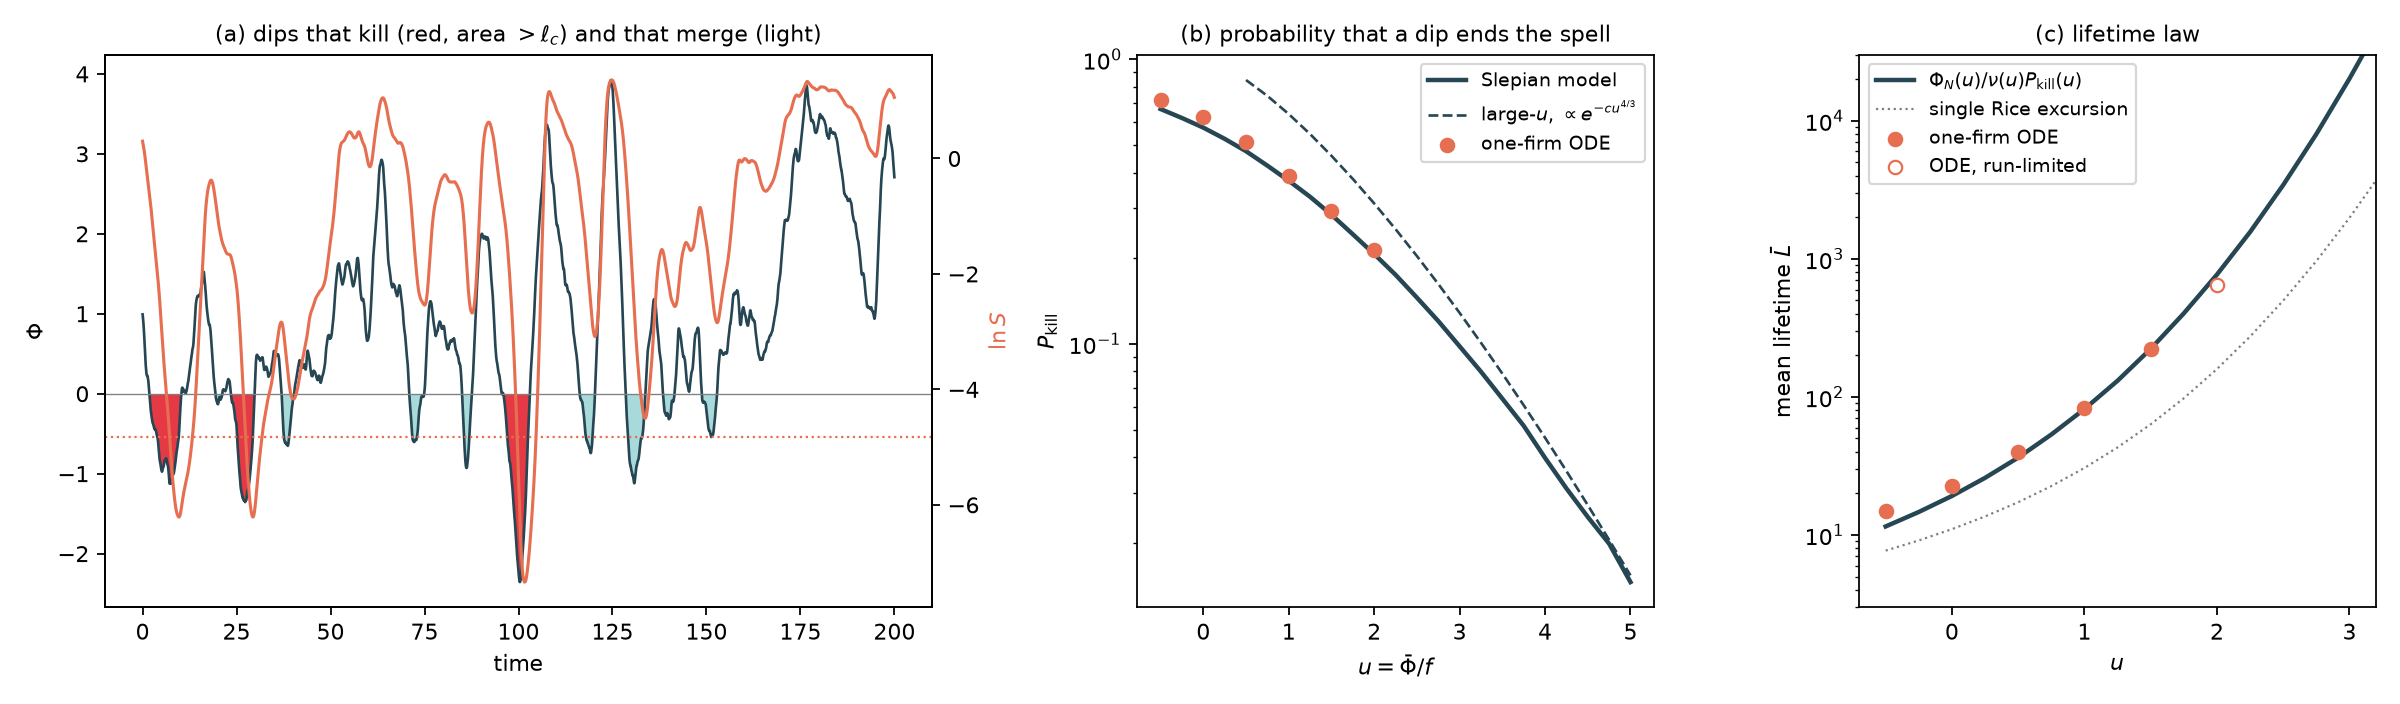
\includegraphics[width=\linewidth]{lifetime_law.png}
  \caption{Kill rule and lifetime law, $\alpha=6$ fitness.  (a) A fitness path with its dips: red dips
  have area above $\ell_c(s)$ and end the spell ($\ln S$, right axis, crosses the threshold, dotted);
  light dips merge neighbouring excursions.  (b) $P_{\rm kill}(u)$ from the one-firm ODE, the Slepian
  model and the large-$u$ asymptote \eqref{eq:largeu}.  (c) Mean lifetime: ODE against
  \eqref{eq:lifetime} with the Slepian $P_{\rm kill}$, and the single-excursion Rice value; the hollow
  point is biased short by the run length.  Source: \texttt{scripts/lifecycle/plot\_lifetime\_law.py}.}
  \label{fig:lifetime}
\end{figure}

Table~\ref{tab:rice} shows three things.  The Slepian $P_{\rm kill}$ is within $0.05$ of the ODE
everywhere and exact for $u\ge1.5$; the deficit at small $u$ is the unrecovered dips.  With no
simulation input, \eqref{eq:lifetime} gives the mean lifetime to $3\%$ for $u\ge1$ and runs
$10$--$20\%$ low for $u\le0.5$, where short spells and the entry and exit delays matter.  And
$\Var\ln L$ rises to $\pi^2/6=1.645$ at $u=1.5$, the value for an exponential law: large firms exit
on rare, memoryless kills, exactly as the crossover argument of the previous subsection assumed.
The asymptotic form \eqref{eq:largeu} sets in only for $u\gtrsim4$, because at moderate $u$ the
killing dips last about $\tau$ and are not parabolic.

Two consequences follow.
\begin{enumerate}
  \item \emph{Lifetime grows faster than any power of size.}  With $\bar S\simeq\bPhi=uf$ for long
        spells, $\ln\bar L$ grows as $\bar S^2/2f^2$ plus a $\bar S^{4/3}$ correction.  Through
        \eqref{eq:lifetimerep} the life-cycle part of the volatility has a local exponent that
        increases along the decline branch, so the spell $\beta$ is an effective exponent whose
        value depends on the fitted size range, and the model's decline branch steepens with size.
  \item \emph{Slow convergence.}  Firms whose lifetime exceeds the panel length $T$ appear as one
        cut-off spell dominated by the plateau ($v\propto1/S$); shorter-lived firms are dominated
        by the rise and fall.  The crossover is at $\bar L(u_\times)\simeq T$, so $u_\times$ grows
        only as $\sqrt{2\ln T}$.  This is why the spell $\beta$ converges slowly in $T$, even
        though it has a limit.
\end{enumerate}

\subsection{The degree channel is amplitude heterogeneity}

At $\alpha=2.5$ the spell ratio curve is flat.  The surrogate isolates the cause:

\begin{center}\small
\begin{tabular}{lcc}
\toprule
$\alpha=2.5$, spells & $\beta$ & $\zeta_q/\zeta_1$\\
\midrule
full model & $0.191$ & $1.42,\,1.34,\,0.95$\\
surrogate, measured $(\bPhi_i,f_i)$ & $0.183$ & $1.49,\,1.61,\,1.52$\\
$f$ shuffled across firms & $0.092$ & $1.40,\,1.47,\,1.31$\\
$f$ homogeneous & $0.493$ & $1.89,\,2.64,\,3.25$\\
\bottomrule
\end{tabular}
\end{center}

\noindent Breaking the link between $\bPhi$ and $f$ keeps the curve flat; removing the spread of
$f$ restores the plain life-cycle bend.  The heavy-tail flattening is the spread of fitness
amplitudes, $f\propto\sqrt\kappa$, which at fixed size adds lifetime dispersion on top of the life
cycle: Proposition~\ref{prop:criterion} with two random factors.  On heavy tails the degree
moments also grow faster than $q$ and lower $\zeta_1$ from $0.29$ to $0.18$, and dividing the
same absolute bend by a smaller $\zeta_1$ flattens the curve further.

\subsection{Closing the chain}

Sampling $(\bPhi,f)$ from Proposition~\ref{prop:law} and running the single-firm process gives the
spell statistics with progressively less simulation input:

\begin{center}\footnotesize\setlength{\tabcolsep}{3pt}
\begin{tabular}{l|c|c|c|c}
\toprule
spells, $T=480$ & full model & measured $(\bPhi_i,f_i)$ & law (sim.\ order par.) & law (HDMFT)\\
\midrule
$\alpha=6$, $\sigma=1.75$   & $0.554$; $1.84,2.50,3.00$ & $0.536$; $1.77,2.33,2.74$ & $0.636$; $1.82,2.45,2.93$ & $0.532$; $1.85,2.53,3.06$\\
$\alpha=3.5$, $\sigma=1.9$  & $0.284$; $1.79,2.30,2.53$ & $0.288$; $1.79,2.37,2.76$ & $0.347$; $1.78,2.34,2.70$ & $0.383$; $1.80,2.41,2.85$\\
$\alpha=2.5$, $\sigma=1.75$ & $0.191$; $1.42,1.34,0.95$ & $0.183$; $1.49,1.61,1.52$ & $0.248$; $1.55,1.73,1.70$ & $0.237$; $1.57,1.80,1.82$\\
\bottomrule
\end{tabular}
\end{center}

\noindent Each entry is $\beta$; $\zeta_q/\zeta_1$ for $q=2,3,4$.  The last column has no simulation
input: the HDMFT solved on the degree sequence gives the order parameters,
Proposition~\ref{prop:law} gives $(\bPhi,f)$, the one-firm process gives the life cycles, and the
MSB estimator is applied to them.  The ratio curve is reproduced at every level of input, to
$0.1$--$0.3$ on light tails.  The level of $\beta$ is more fragile.  With the simulation's own order
parameters the law gives a $\beta$ $0.06$--$0.10$ above the full model, because the leading-order
law lacks the $\pm13\%$ spread of amplitudes at fixed degree (Table~\ref{tab:cavity}) that comes from
quenched neighbourhoods; less amplitude spread means less flattening and a steeper decline.  With
the HDMFT order parameters, which are within about $10\%$ of the simulated ones, $\beta$ lands within
$0.02$ of the full model at $\alpha=6$ and $0.10$ at $\alpha=3.5$; the close agreement at $\alpha=6$ is
partly a cancellation and should not be over-read.

\subsection{Where the model meets the data}
\label{sec:data}

\paragraph{Estimator.}  On the spell panel the binned volatility has a hump at small sizes, made of
spells that barely clear the listing threshold, and a flat top.  A fit that starts at the peak
bin is unstable: the start moves by a bin between economies and $\beta$ jumps by up to $0.09$.  We
therefore fit every exponent on the larger half of spells by $\bar S$, in ten equal-count bins of
$v^q$ (\texttt{msb.upper\_zeta}).  The range is fixed by spell counts, so $\beta$ varies by $\pm0.03$
between economies.  All spell-panel tables use this estimator; the window-convergence
values quoted in Section~\ref{sec:panels} and the survivor panel use the peak-start fit of the
original analysis, with which $\beta$ is $0.07$--$0.14$ lower and the ratios differ by at most $0.06$.

\paragraph{Shape against level.}  Figure~\ref{fig:data} and the table below give the full model at
four points.  The ratio curve is robust: it does not depend on the estimator, and on light tails
it is close to the data, $1.84$, $2.50$, $3.00$ at $\alpha=6$ against $2.0$, $2.6$, $2.9$.  Its bend is
the life-cycle mechanism of this section.  The level of $\beta$ is not robust.  It depends on the
fitted size range, because the decline branch steepens with size (Figure~\ref{fig:data}a, as the
lifetime law of Section~\ref{sec:rice} predicts), and on the entry size, which sets the rise term
$\ell$.  With the fixed range no point gives $\beta\approx0.2$ together with data-like ratios: light
tails give data-like ratios with $\beta=0.55$, heavy tails give $\beta\approx0.2$ with a flat or falling
ratio curve, the result of amplitude heterogeneity.  The model therefore accounts for the shape of
the multiscaling and for a size--volatility law of the right sign, but not for the empirical
value of $\beta$ under a protocol-matched estimator.  The empirical curve flattens at the top,
while the model's steepens; we read this as the main quantitative mismatch.

\begin{center}\small\setlength{\tabcolsep}{5pt}
\begin{tabular}{l|cc|cc}
\toprule
full model, spells, $T=480$ & $\beta$ (fixed range) & $\zeta_q/\zeta_1$ & $\beta$ (peak start) & $\zeta_q/\zeta_1$\\
\midrule
$\alpha=6$, $\sigma=1.75$, $\lambda=10^{-3}$ & $0.55\pm0.03$ & $1.84,\,2.50,\,3.00$ & $0.42$ & $1.86,\,2.55,\,3.07$\\
$\alpha=3.5$, $\sigma=1.9$, $\lambda=10^{-3}$ & $0.28\pm0.03$ & $1.79,\,2.30,\,2.53$ & $0.20$ & $1.80,\,2.31,\,2.54$\\
$\alpha=3.5$, $\sigma=1.9$, $\lambda=10^{-2}$ & $0.30\pm0.03$ & $1.79,\,2.27,\,2.39$ & $0.23$ & $1.78,\,2.24,\,2.32$\\
$\alpha=2.5$, $\sigma=1.75$, $\lambda=10^{-3}$ & $0.19$ & $1.42,\,1.34,\,0.95$ & $0.16$ & $1.49,\,1.48,\,1.14$\\
\midrule
Compustat & $0.15$--$0.20$ & $2.0,\,2.6,\,2.9$ & & \\
\bottomrule
\end{tabular}
\end{center}

\noindent Medians over eight economies, $N=8000$, $C=200$, $\mu=-1.76$, spells of at least two growth
rates.  Across the earlier $36$-point scan the growth rates stay fat-tailed (excess kurtosis
$3$--$16$).  Sources: \texttt{scripts/headline\_spells.py}, \texttt{scripts/plot\_data\_comparison.py}.

\begin{figure}[htbp]
  \centering
  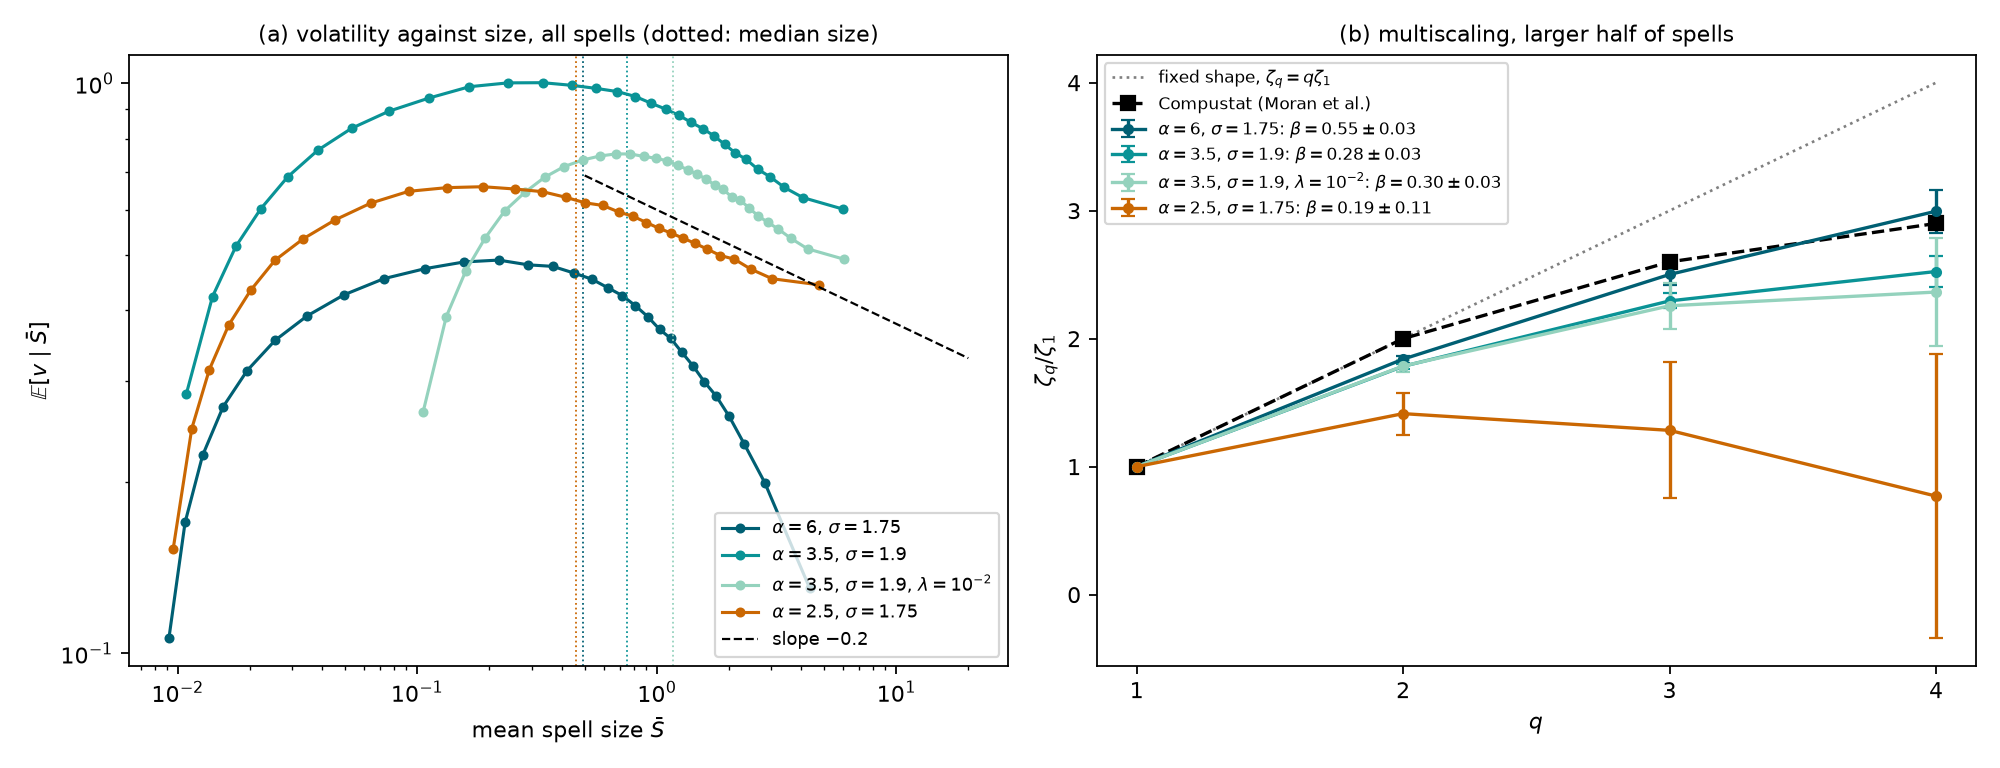
\includegraphics[width=\linewidth]{data_comparison.png}
  \caption{Full model under the spell panel against the empirical facts.  (a) $\E[v\mid\bar S]$ over
  all spells, pooled over eight economies; the fixed estimator fits the larger half of spells
  (right of the dotted line).  The decline branch steepens with size.  (b) $\zeta_q/\zeta_1$ with the
  fixed estimator (mean and spread over economies), the Compustat values of \citet{moran2024} and
  the fixed-shape line.}
  \label{fig:data}
\end{figure}

%======================================================================
\section{Discussion}
\label{sec:discussion}

\paragraph{The picture.}
Scale invariance turns the economy into a replicator in which each firm is a logistic unit
tracking a fitness field.  Mean-field theory makes that field Gaussian, with mean and amplitude
set by the degree, and organises the phase diagram.  Below the stability line the economy has a
unique frozen composition; degree heterogeneity lowers the line, a mean interaction of either
sign raises it, and competition, which removes the noisiest firms, raises it most.  Above the
line the composition is chaotic or trapped by one of many equilibria, and the growth boundary is
almost independent of the network.  In the fluctuating, growing phase every firm is an
independent one-dimensional problem with a known law of parameters.  The empirical protocol counts
whole lives, and a firm's volatility is then its log range over its lifetime: it enters when its
fitness has risen enough, exits on the first fitness dip whose area exceeds an explicit threshold,
and in between is one hump or a few merged ones.  The empirical exponents are therefore lifetime
exponents, and the bend of the ratio curve is the growing spread of lifetimes with size: regular
single excursions for small firms, memoryless exits for large ones.  The bend is a crossover.  In
this model multiscaling is an effective property of a finite size range, not an asymptotic law,
consistent with the reading of \citet{moran2024}.  The plateau mechanism (an adiabatic
$\sqrt D/S$ law and a degree channel, Appendices~\ref{sec:adiabatic}--\ref{sec:survivor}) governs only
firms present throughout a window.

\paragraph{Predictions for data.}
\begin{enumerate}
  \item \emph{Survivorship.}  Restricting a panel to firms present throughout should raise $\beta$
        (in the model, $0.41$ against $0.20$ at $\alpha=2.5$).
  \item \emph{Lifetime bound.}  Eq.~\eqref{eq:bound} bounds each firm's volatility from below by
        its life-cycle range and lifetime.  The MSB growth rates are overlapping annual differences
        sampled quarterly, so the bound must be adapted to that sampling before the test.
  \item \emph{Age.}  Removing each firm's entry and exit years, or conditioning on age, should move
        $\zeta_q/\zeta_1$ towards $q$.
\end{enumerate}

\subsection{Open problems}
\label{sec:open}
\begin{itemize}
  \item \emph{Growth in the fluctuating phase.}  The zero-growth line agrees with simulation only
        as the continuation of an unstable fixed point; the controlled condition $\bar g=0$ needs
        the two-time theory.  In the coexistence region above $\sigma_c$ the trapping probability
        grows with the observation time (Section~\ref{sec:above}); its dependence on $N$ and $T$,
        and whether trapping survives $N\to\infty$, is not mapped.
  \item \emph{Light-tail $\bad$.}  Linear response is $0.09$--$0.12$ low on light tails; the
        nonlinear one-firm response is not derived.
  \item \emph{Sparse cavity.}  At $\alpha\lesssim2.2$ the field is carried by about four neighbours
        and is not Gaussian.  A few-neighbour cavity theory is needed.
  \item \emph{Finite connectivity.}  The spread of amplitudes at fixed degree, which comes from
        quenched neighbourhoods, is not derived.  It controls $\varepsilon_C$ on the survivor panel and
        the extra flattening on the spell panel, and its $N$ dependence sets the slow approach to
        the limit.
  \item \emph{A full spell theory.}  Spells are humps merged by non-killing dips
        (Section~\ref{sec:humps}), and this gives each spell's volatility to $4$--$10\%$, but not yet
        the exponents: the largest firms carry extra variation from fitness fluctuations that never
        reach zero.  The lifetime law \eqref{eq:lifetime} also misses the shortest spells and the
        dips that start before the firm has recovered.  With these, the $(\bPhi,f)$ ensemble would
        give $\zeta_q$ analytically.
  \item \emph{Entry size.}  Model firms enter at $\Sthr\approx10^{-2}$ of the mean size and rise by
        $e^\ell\sim e^5$; real firms enter Compustat at their IPO size.  The model probably
        overstates the rise-and-fall share; the entry size should be calibrated from data rather
        than treated as a free parameter.
\end{itemize}

\appendix
%======================================================================
\section{Plateau volatility: the adiabatic law}
\label{sec:adiabatic}

\paragraph{Observables.}
Fix a horizon $\Delta t$ ($0.5$ in production) and let $G_i=\ln S_i(t+\Delta t)-\ln S_i(t)$.  The
volatility $v_i$ is the MAD estimate $\sqrt{\pi/2}\,\overline{|G_i-\bar G_i|}$, and $\bar S_i$ the
mean size.  The local exponent is $\beta(S)=-d\ln\E[v\mid\bar S=S]/d\ln S$; the reported $\beta$ is
its least-squares average over the decline branch, and $\zeta_q$ is defined in the same way from
$\E[v^q\mid\bar S]$.

\subsection{The adiabatic law}
\label{sec:adlaw}

\begin{proposition}[Adiabatic volatility law; leading order]\label{prop:adiabatic}
Linearise \eqref{eq:firm} about the firm's mean size, $S=\bar S(1+u)$, at $\lambda\to0$.  Then
$\dot u=-\bar Su+\delta\Phi$: the log-size is the fitness passed through a low-pass filter
$1/(\bar S+i\omega)$, and
\begin{equation}
  v^2=\sigma^2\kappa\,A^2(\bar S),\qquad
  A^2(S)=\int\frac{d\omega}{2\pi}\,\frac{4\sin^2(\omega\Delta t/2)\,\widehat Q(\omega)}{S^2+\omega^2},
  \label{eq:A}
\end{equation}
where $\widehat Q$ is the spectrum of the fluctuating part of $\xi$.  $A$ does not depend on
$\kappa$.
\end{proposition}
The exponent $\beta_A=-d\ln A/d\ln S$ has three regimes, set by the correlation rate $\omega_c$
of the field and by the horizon.
\begin{enumerate}
  \item $S\gg\omega_c$ and $S\Delta t\gg1$ (adiabatic).  The firm tracks its fitness,
        $\ln S\approx\ln\Phi$, so
        \begin{equation}
          v=\frac{\sqrt D}{S},\qquad D=\Var[\Phi(t+\Delta t)-\Phi(t)],\qquad\beta_A=1 .
          \label{eq:adlimit}
        \end{equation}
        This needs only the separation of time scales, not linearity, so it holds firm by firm
        with $D_i$ the realised increment variance of that firm's field.
  \item $\omega_c\ll S\ll\Delta t^{-1}$ with a rough field ($\widehat Q\sim\omega^{-2}$):
        $A^2\propto S^{-1}$ and $\beta_A=\tfrac12$.
  \item $S\ll\omega_c$: the firm integrates the field without relaxing, $A$ is flat and
        $\beta_A=0$.  The floor sits here.
\end{enumerate}

\begin{corollary}[Homogeneous graphs]\label{cor:homog}
If $\kappa\equiv1$, $\beta=\beta_A$, and $\beta\to1$ as the fit window moves into regime~1.
\end{corollary}
In simulation $\beta=1.02$ on the fully connected graph and $0.99$ on the regular graph at
$N=32000$.  Raising $\Delta t$ moves a fixed size window from regime~2 towards regime~1, so
$\beta$ grows with the horizon, as observed.  The $\sqrt\kappa$ prefactor is quantitative: at
$N=16000$, $\alpha=2.5$, $vS/\sqrt k$ binned in size agrees across degree quartiles to a few per
cent, and a joint regression $\ln v=c-a\ln S+b\ln k$ gives $b=0.50\pm0.03$ ($0.42$--$0.54$ for
every $\alpha$).

\subsection{The adiabatic slope from the two-time HDMFT}

Define $\bad$ as the slope of the volatility normalised by each firm's realised fitness
amplitude, $-d\ln\E[v/\sqrt{D_i}\mid\bar S]/d\ln\bar S$.  Driving \eqref{eq:firm} with a firm's own
measured $\Phi_i(t)$ reproduces it to within $0.005$ on every graph, so $\bad$ is a property of
the one-firm process and the law of its field.  The two-time HDMFT predicts it to within $0.035$
on every graph, including $\alpha=2.2$ (Table~\ref{tab:beta}, first two columns).

What varies across graphs is the \emph{roughness} of the field, the ratio of the increment
variance to the variance.  Replacing each firm's own spectrum by the average spectrum of the
decline branch changes the linear-response $\bad$ by at most $0.012$, so the shape is not
firm-specific.  In the diagonal, annealed approximation
\begin{equation}
  \frac{\Var[\Delta h]}{\Var[h]}\simeq\frac{\E_w[d_j]}{\E_w[\Var_tS_j]},\qquad
  d_j=\Var[S_j(t+\Delta t)-S_j(t)],\quad w_j\propto k_j ,
  \label{eq:rough}
\end{equation}
which gives $0.408$, $0.073$, $0.056$, $0.030$ against measured $0.429$, $0.088$, $0.068$, $0.036$
for $\alpha=2.2$, $2.5$, $3.5$, $6$.  Heavy tails roughen the field because neighbours are drawn in
proportion to degree, surviving hubs are large, and large firms relax fast, at rate $\bar S_j$, so
they carry the high frequencies.  A rough field pushes firms at the start of the decline branch,
where $\bar S\Delta t\approx0.5$, out of the adiabatic regime, and $\bad$ falls.

Linear response gets the number only on heavy tails.  With the survivors' own fitness paths it
gives $0.688$ and $0.746$ against $0.680$ and $0.782$ at $\alpha=2.2$ and $2.5$, but runs
$0.09$--$0.12$ low on light tails, where it cannot exceed one while the measurement reaches
$1.01$.  The light-tail gap is a nonlinear one-firm effect, not yet derived.

%======================================================================
\section{The survivor panel and the degree channel}
\label{sec:survivor}

\subsection{Sum rule}
\label{sec:sumrule}

\begin{proposition}[Sum rule]\label{prop:sum}
If $v/\sqrt\kappa$ is independent of $\kappa$ given $\bar S$, then, exactly,
\begin{equation}
  \beta(S)=\beta_A(S)-\varepsilon_k(S),\qquad
  \beta_A=-\frac{d\ln\E[v/\sqrt\kappa\mid\bar S=S]}{d\ln S},\qquad
  \varepsilon_k=\frac{d\ln\E[\sqrt\kappa\mid\bar S=S]}{d\ln S}.
  \label{eq:sum}
\end{equation}
At leading order $\beta_A$ is the slope of $A(\bar S)$ in \eqref{eq:A} plus any size dependence of
the residual factor.
\end{proposition}
A graph lowers $\beta$ only to the extent that larger firms sit on larger degrees.  The size of
the degree heterogeneity does not matter on its own; what matters is how strongly size selects on
it.  Integrating \eqref{eq:sum} gives a fixed budget,
$\int[\beta_A-\beta]\,d\ln S=\ln\bigl(\E[\sqrt\kappa\mid S\to\infty]/\E[\sqrt\kappa\mid S\to0]\bigr)\le
\tfrac12\ln(\kappa_{\max}/\kappa_{\min})$.  At fixed dilution $C=N/40$ the degree range does not grow
with $N$, so the degree channel alone cannot send $\beta\to0$ as $N\to\infty$.

In simulation the sum rule holds to within $0.04$ on every graph ($\beta$, $\beta_A$, $\varepsilon_k$
$=0.414$, $0.581$, $0.174$ at $\alpha=2.5$; $0.894$, $0.916$, $0.034$ at $\alpha=6$; full values in
Table~\ref{tab:beta}).  Most of the topology dependence is in $\beta_A$, not in $\varepsilon_k$: at
$\alpha=2.2$, $1-\beta_A=0.56$ against $\varepsilon_k=0.23$.

\subsection{The survivor ensemble}
\label{sec:ensemble}

$\varepsilon_k$ is a property of which firms survive the window.  At leading order it follows
from three ingredients, each checked inside the HDMFT on paths whose fitness was reconstructed
exactly:
\begin{enumerate}
  \item size is mean fitness, $\bar S=\bPhi$ (Proposition~\ref{prop:size});
  \item at fixed degree the window-mean fitness is Gaussian, $\bPhi=r_\kappa+a_\kappa x$ with
        fluctuations of amplitude $f_\kappa$ around it (Proposition~\ref{prop:law});
  \item survival is an extreme-value event: a firm survives if its mean fitness exceeds its
        deepest dip.  With $b=T/2\tau$ roughly independent blocks in the window,
        \begin{equation}
          P_{\rm surv}(u)=\PhiN(u)^{\,b},\qquad u=\frac{\bPhi}{f_\kappa}.
          \label{eq:ev}
        \end{equation}
\end{enumerate}
The survival curve depends on $u$ alone and is the same at low and high degree:

\begin{center}\small
\begin{tabular}{lcccccccc}
\toprule
$u=\bPhi/f_\kappa$ & 0 & 0.25 & 0.5 & 0.75 & 1.0 & 1.25 & 1.5 & 1.75\\
\midrule
low-degree half  & 0.00 & 0.01 & 0.07 & 0.25 & 0.38 & 0.61 & 0.84 & 0.92\\
high-degree half & 0.00 & 0.01 & 0.07 & 0.21 & 0.32 & 0.55 & 0.77 & 0.82\\
\bottomrule
\end{tabular}
\end{center}

\noindent Its soft shape is that of \eqref{eq:ev} with $b\approx9$ ($\alpha=3.5$, $T=60$, $\tau=3.4$).
Two simpler laws fail.  A sharp level crossing gives the right scaling in $f_\kappa$ but a hard
threshold, which misses the survivors just below it; these set the low tail of the size
distribution, and dropping them nearly doubles $\varepsilon_k$ (to $0.41$ at $\alpha=2.5$).  A drawdown law gives a threshold
$\propto f_\kappa^2$, the wrong scaling.

\paragraph{The degree channel.}  Among survivors the joint law of degree and size is explicit,
\begin{equation}
  p(\kappa,S)\propto p(\kappa)\,\frac1{a_\kappa}\,\phiN\!\left(\frac{S-r_\kappa}{a_\kappa}\right)
  \PhiN\!\left(\frac S{f_\kappa}\right)^{b},
  \label{eq:joint}
\end{equation}
and $\varepsilon_k$ follows by one quadrature over $\kappa$ at each $S$.  Differentiating,
\begin{equation}
  \varepsilon_k(S)=\frac{S\,\Cov_{\kappa\mid S}\bigl(\sqrt\kappa,\;\partial_S\ln p\bigr)}{\E[\sqrt\kappa\mid S]},
  \qquad
  \partial_S\ln p=-\frac{S-r_\kappa}{a_\kappa^2}+\frac{b}{f_\kappa}\,\frac{\phiN(S/f_\kappa)}{\PhiN(S/f_\kappa)}.
  \label{eq:epscov}
\end{equation}
Two forces act on the degree of a firm of given size.  The first term is the Gaussian cost of
reaching $S$, cheaper for large $a_\kappa\propto\sqrt\kappa$, so large firms are drawn to high degree;
the load $\mu\kappa\bar B$ in $r_\kappa$ pushes the other way.  The second is the survival pressure,
which acts near the threshold.  Since the threshold is in units of $f_\kappa\propto\sqrt\kappa$,
surviving sizes scale close to $\sqrt\kappa$ whatever the load: \eqref{eq:joint} gives
$\bar S\propto k^{\delta}$ with $\delta=0.40$, against $0.43$--$0.51$ in the HDMFT and $0.47$--$0.52$
in simulation.

The inputs are the HDMFT order parameters, $\tau$, the degree law and $T$; nothing is fitted to
$\beta$.  Against the HDMFT's own survivors the ensemble runs $10$--$30\%$ low on the survival
fraction but reproduces the degree channel and the size spread to within $0.015$ for
$\alpha\ge2.5$:

\begin{center}\small\setlength{\tabcolsep}{4pt}
\begin{tabular}{lcc|cc|cc|cc}
\toprule
$\alpha$ & $\tau$ & $b$ & surv HD & surv \eqref{eq:ev} & $\varepsilon_k$ HD & $\varepsilon_k$ \eqref{eq:joint} & $\Var\ln S$ HD & $\Var\ln S$ \eqref{eq:joint}\\
\midrule
2.2 & 2.41 & 12.4 & 0.139 & 0.094 & 0.287 & 0.332 & 0.149 & 0.140\\
2.5 & 2.73 & 11.0 & 0.124 & 0.096 & 0.220 & 0.235 & 0.157 & 0.156\\
3.5 & 3.38 & 8.9  & 0.148 & 0.133 & 0.111 & 0.115 & 0.170 & 0.174\\
6.0 & 3.62 & 8.3  & 0.175 & 0.152 & 0.036 & 0.035 & 0.174 & 0.180\\
\bottomrule
\end{tabular}
\end{center}

\paragraph{The window enters.}  Through $b=T/2\tau$ and $Q_T$, \eqref{eq:joint} depends on $T$: a
longer window is a stricter survival test, survivors are selected further out in the size tail,
and $\varepsilon_k$ grows.  Simulation confirms it ($\varepsilon_k=0.132$, $0.179$, $0.201$ at
$T=30$, $60$, $120$, $\alpha=2.5$).  This is the formal reason the survivor panel has no
long-window limit: its exponent is tied to the analyst's window.  The survivor numbers below are
at $T=60$.

\subsection{Finite connectivity}
\label{sec:finiteC}

The HDMFT replaces each firm's neighbourhood by its degree class.  In a finite graph the field is
a quenched sum over actual neighbours, and its increment variance is, to within $1$--$5\%$,
$D_i\simeq(\sigma^2/C)\sum_jA_{ij}z_{ij}^2d_j$.  What matters is how few neighbours carry the sum:
the effective number $n_{\rm eff}=(\sum_jc_j)^2/\sum_jc_j^2$, $c_j=z_{ij}^2d_j$, is $24$ at $\alpha=6$
and only $4$ at $\alpha=2.2$.

The same neighbours and couplings set the firm's static field, hence its size
(Proposition~\ref{prop:size}).  A firm that is large because it drew large neighbours or
favourable couplings to them also has a large volatility amplitude.  We estimate, without a derivation, that this within-class selection
lowers $\beta$ by an amount proportional to $c_{ds}\E[k^{-1}]$, the inverse effective number of
neighbours weighted by $c_{ds}=\E_w[d\bar S^2]/(\E_w[d]\,\E_w[\bar S^2])$, which measures how much the
neighbours that carry the size also carry the noise.  $c_{ds}$ grows with the degree tail, from
$3.4$ at $\alpha=6$ to $6.3$ at $\alpha=2.2$; on homogeneous graphs $c_{ds}\to1$ and the correction
is $O(1/C)$.

The correction can be read off directly.  Normalising by the realised amplitude $D_i$ removes it;
normalising by $\sqrt\kappa$ does not.  Define $\varepsilon_C:=\bad-\varepsilon_\chi-\beta_A$ in simulation.  Using the sum rule on both sides,
\[
  \beta^{\rm HD}-\beta^{\rm sim}=\varepsilon_C+\bigl(\bad^{\rm HD}-\bad^{\rm sim}\bigr)
  +\bigl(\varepsilon_k^{\rm sim}-\varepsilon_k^{\rm HD}\bigr)+\delta_{\rm sum},
\]
where $\delta_{\rm sum}$ collects the residuals of the sum rule ($\le0.04$).  The two brackets are
at most $0.04$ in Table~\ref{tab:beta}, so the gap should track $\varepsilon_C$ to within a few
hundredths, and it does (last two columns).  Here $\varepsilon_\chi=0.02$--$0.03$ is the slope of the ratio of realised to
class amplitude inside the HDMFT: near-threshold survivors are those whose realised fluctuations
happened to be small.

The approach to $N\to\infty$ is slow.  At $\alpha=2.5$ the gap goes from $0.15$ at $N=8000$ to $0.14$
at $N=16000$, although $\E[k^{-1}]$ halves: $c_{ds}$ grows with the heaviest neighbour weights
($4.6\to5.5$), and $\varepsilon_k$ approaches its HDMFT value from below ($0.174\to0.213$, against
$0.214$).  The approach is not linear in $1/N$, and extrapolations that assume it are not a sharp
test.

\subsection{Assembled exponent}

At leading order the exponent is the HDMFT's, and the survivor ensemble gives it analytically,
\begin{equation}
  \beta_\infty\simeq\bad-\varepsilon_\chi-\varepsilon_k ,
  \label{eq:betainf}
\end{equation}
with $\varepsilon_k$ from \eqref{eq:joint} and $\bad$, $\varepsilon_\chi$ from the one-firm process.
Finite connectivity then subtracts $\varepsilon_C$.

\begin{table}[htbp]
\centering\small\setlength{\tabcolsep}{3.5pt}
\begin{tabular}{l|cc|ccc|cc|ccc|cc}
\toprule
$\alpha$ & $\bad^{\rm HD}$ & $\bad^{\rm sim}$ & $\varepsilon_\chi$ & $\varepsilon_k^{\rm ens}$ & $\beta_\infty$ \eqref{eq:betainf}
 & $\beta^{\rm HD}$ & $\varepsilon_k^{\rm HD}$ & $\beta^{\rm sim}$ & $\beta_A^{\rm sim}$ & $\varepsilon_k^{\rm sim}$
 & $\varepsilon_C^{\rm sim}$ & $\beta^{\rm HD}-\beta^{\rm sim}$\\
\midrule
2.2 & 0.680 & 0.697 & 0.029 & 0.332 & 0.320 & 0.397 & 0.268 & 0.209 & 0.440 & 0.229 & 0.23 & (0.19)\\
2.5 & 0.782 & 0.749 & 0.028 & 0.235 & 0.519 & 0.566 & 0.214 & 0.414 & 0.581 & 0.174 & 0.14 & 0.15\\
3.5 & 0.937 & 0.918 & 0.025 & 0.115 & 0.797 & 0.826 & 0.109 & 0.691 & 0.788 & 0.102 & 0.11 & 0.14\\
6.0 & 0.987 & 1.014 & 0.019 & 0.035 & 0.933 & 0.945 & 0.035 & 0.894 & 0.916 & 0.034 & 0.08 & 0.05\\
\bottomrule
\end{tabular}
\caption{The survivor-panel exponent, $N=8000$, $C=200$, $(\mu,\sigma,\lambda)=(-1.76,1.75,10^{-3})$,
$T=60$.  Simulation values are medians over eight economies (seven at $\alpha=2.2$).
$\varepsilon_C^{\rm sim}=\bad^{\rm sim}-\varepsilon_\chi-\beta_A^{\rm sim}$.  The HDMFT does not converge
at $\alpha=2.2$, so the bracketed gap should not be used.}
\label{tab:beta}
\end{table}

The analytic form runs $0.01$--$0.08$ below $\beta^{\rm HD}$, because the ensemble overestimates
$\varepsilon_k$ on heavy tails and the split holds inside the HDMFT only to $0.03$.  At $\alpha=2.2$
only $\bad$, which the HDMFT still gets right, should be trusted.

\subsection{Multiscaling from degree}

With $X=\sqrt\kappa$ the split of the moments is $\zeta_q=\zeta_q^A-e_q$, with
$e_q=d\ln\E[\kappa^{q/2}\mid S]/d\ln S$ and $\zeta_q^A$ the exponents of $v/\sqrt\kappa$, and
\begin{equation}
  q-\frac{\zeta_q}{\zeta_1}=\frac{(e_q-q\,e_1)+(q\,\zeta_1^A-\zeta_q^A)}{\zeta_1}.
  \label{eq:bend}
\end{equation}
The bend has two sources, a superlinear degree moment and a degree-normalised volatility not of
fixed shape, and both are amplified by a small $\zeta_1=\beta$.  By
Proposition~\ref{prop:criterion}, the first is nonzero only if $\Var(\ln\kappa\mid S)$ grows with
$S$.  A log-normal joint law of $(\kappa,S)$ has constant conditional variance and gives no bend;
the survivor ensemble does not.

Take the load small and $a_\kappa=a_1\sqrt\kappa$, $f_\kappa=f_1\sqrt\kappa$.  For a Pareto degree law on
$[\kappa_{\min},\kappa_{\max}]$, change variable in \eqref{eq:joint} to $u=S/\sqrt\kappa$:
\begin{equation}
  p(u\mid S)\propto u^{2\alpha-2}\,\phiN\!\left(\frac u{a_1}\right)\PhiN\!\left(\frac u{f_1}\right)^{b},
  \qquad\frac S{\sqrt{\kappa_{\max}}}<u<\frac S{\sqrt{\kappa_{\min}}} ,
\end{equation}
and $\E[\kappa^{q/2}\mid S]=S^q\E[u^{-q}\mid S]$.  Size enters only through the edges of the support.
Without cutoffs $u$ is independent of $S$, $e_q=q$ and there is no bend: size is pure amplitude.
The lower cutoff pins the smallest survivors to $\kappa_{\min}$, where the conditional spread
vanishes; as $S$ grows the edge $S/\sqrt{\kappa_{\min}}$ moves through the bulk, the admissible
degrees open, and the spread rises to its unconstrained value.  The upper cutoff carries no
weight, because hubs of a given size do not survive (the survival factor tends to $2^{-b}$).  The
degree bend is therefore a crossover, living on the range of sizes over which the lower cutoff
releases.

\begin{table}[htbp]
\centering\small\setlength{\tabcolsep}{4pt}
\begin{tabular}{l|ccc|cc|cc|ccc}
\toprule
 & \multicolumn{3}{c|}{$e_4/e_1$} & \multicolumn{2}{c|}{$\zeta_4^A/\zeta_1^A$} & \multicolumn{2}{c|}{$e_1/\zeta_1$}
 & \multicolumn{3}{c}{$\zeta_q/\zeta_1$, $q=2,3,4$}\\
$\alpha$ & HD & ens. & sim & HD & sim & HD & sim & HDMFT & $\zeta_q^{A,\rm HD}-e_q^{\rm ens}$ & simulation\\
\midrule
2.2 & 4.88 & 5.59 & 5.45 & 3.90 & 3.68 & 0.80 & 1.25 & 1.79, 2.40, 2.87 & 1.80, 2.28, 2.19 & 1.86, 2.51, 3.01\\
2.5 & 5.29 & 6.15 & 5.69 & 3.87 & 3.73 & 0.42 & 0.48 & 1.86, 2.60, 3.23 & 1.85, 2.48, 2.79 & 1.88, 2.63, 3.20\\
3.5 & 5.92 & 6.38 & 5.40 & 3.96 & 3.80 & 0.15 & 0.16 & 1.93, 2.79, 3.55 & 1.95, 2.84, 3.61 & 1.94, 2.80, 3.60\\
6.0 & 5.47 & 5.40 & 5.15 & 3.98 & 3.87 & 0.04 & 0.04 & 1.98, 2.94, 3.88 & 1.99, 2.97, 3.93 & 1.96, 2.87, 3.73\\
\bottomrule
\end{tabular}
\caption{Survivor-panel multiscaling.  Fixed-shape values of the two $q=4$ ratios are $4$.  Same
runs as Table~\ref{tab:beta}.  Data: $2.0$, $2.6$, $2.9$.}
\label{tab:zeta}
\end{table}

Table~\ref{tab:zeta} shows that at leading order the bend is all degree: in the HDMFT
$\zeta_4^A/\zeta_1^A$ stays within $0.13$ of $4$, while $e_4/e_1$ exceeds it by $0.9$--$1.9$.  The
HDMFT reproduces the simulated ratio curve to within $0.05$ for $\alpha=2.5$ and $3.5$; the ensemble,
with no simulation input, follows it through $q=3$ and overshoots $e_4$ on heavy tails, where the
fourth moment is carried by coarsely binned top classes.  The ratio curve is a leading-order
property and $\beta$ is not: the HDMFT is off in $\zeta_1$ by $0.14$ at $\alpha=2.5$ and still gets
the ratios right, consistent with the ratios converging in $N$ while $\beta$ drifts.  In simulation
part of the bend also comes from the spread of amplitudes within a class ($\zeta_4^A/\zeta_1^A=
3.68$--$3.87$), so simulation and HDMFT reach nearly the same curve by slightly different routes.

%======================================================================
\section{Gaussian integrals}
\label{app:gauss}

With $\Dz=e^{-z^2/2}dz/\sqrt{2\pi}$ and $w_n(\Delta)=\int_{-\Delta}^\infty\Dz\,(\Delta+z)^n$,
\begin{equation}
  w_0=\PhiN(\Delta),\qquad w_1=\Delta\PhiN(\Delta)+\phiN(\Delta),\qquad
  w_2=(1+\Delta^2)\PhiN(\Delta)+\Delta\phiN(\Delta).
\end{equation}
$w_0=w_2$ only at $\Delta=0$, where $w_0=w_2=\tfrac12$ and $w_1=1/\sqrt{2\pi}$.

\section{Numerics and resolution}
\label{app:numerics}

\paragraph{Resolution.}  A chaotic trajectory does not survive a change of integration tolerance,
so re-integrating the same economies at $10^{-6}$ instead of $10^{-4}$ resamples the late window.
Eight-economy medians of $\beta$ and $\bad$ then move by up to $0.05$ and $0.07$.  On spell panels
a fit that starts at the peak of the binned volatility moves by a bin between economies and
changes $\beta$ by up to $0.09$; the fixed-range estimator of Section~\ref{sec:data} reduces the
spread to $\pm0.03$.  Ratios $\zeta_q/\zeta_1$ are considerably more stable than $\beta$ under any of
these choices.

\paragraph{Sources.}  Scripts are in \texttt{scripts/} unless a path is given.
\begin{center}\small
\begin{tabular}{p{0.42\textwidth}p{0.5\textwidth}}
\toprule
result & script\\
\midrule
fixed-point HDMFT, onset, zero-growth line & \texttt{relative\_glv/hdmft.py}, \texttt{plot\_hdmft\_zero\_growth.py}\\
sum rule, survivor numbers & \texttt{beta\_theory.py}\\
survivor ensemble, $\varepsilon_k$, $\varepsilon_\chi$ & \texttt{beta\_survivor\_theory.py}\\
$\bad$: two-time HDMFT, simulation & \texttt{beta\_ad\_hdmft.py}, \texttt{beta\_ad\_estimators.py}\\
survivor multiscaling & \texttt{zeta\_survivor\_theory.py}\\
fitness statistics and law & \texttt{lifecycle/}: \texttt{fitness\_stats}, \texttt{mf\_law}, \texttt{listed\_by\_degree}\\
surrogate & \texttt{lifecycle/}: \texttt{surrogate}, \texttt{survivor\_check}, \texttt{window\_surrogate}\\
lifetimes, kill rule, ablation & \texttt{lifecycle/}: \texttt{lifetime}, \texttt{kill\_rule}, \texttt{ablation}\\
spell panel, parameter scan & \texttt{beta\_spells.py}, \texttt{scan\_spells.py}\\
headline numbers, data figure & \texttt{headline\_spells.py}, \texttt{plot\_data\_comparison.py}\\
phase diagram & \texttt{phase\_*.py}, \texttt{plot\_phase\_theory.py}\\
fitness-law and lifetime figures & \texttt{lifecycle/}: \texttt{plot\_fitness\_law}, \texttt{plot\_lifetime\_law}\\
\bottomrule
\end{tabular}
\end{center}

\printbibliography[heading=bibintoc]

\end{document}
